\chapter{User Interfaces}

So far we have worked hard on the core mechanic of our game. Another important
aspect are the screens and components that wrap this mechanic. In this chapter
you will learn how to implement menus, popups and other user interface elements
in \cocos{}. 

\cocos{} provides its own set of basic UI components, such as buttons and
labels. For most games these components are sufficient. However, in this chapter
we also learn how to integrate Apple's UI framework \textit{UIKit}. Knowing
that is important for integrating many core Apple API's. As a specific example,
we will add integrate the Game Center framework in this chapter.

By the end of this chapter we will have a fully functional game!
Here's the basic screen flow our game will have:

\begin{figure}[H]
		\centering
		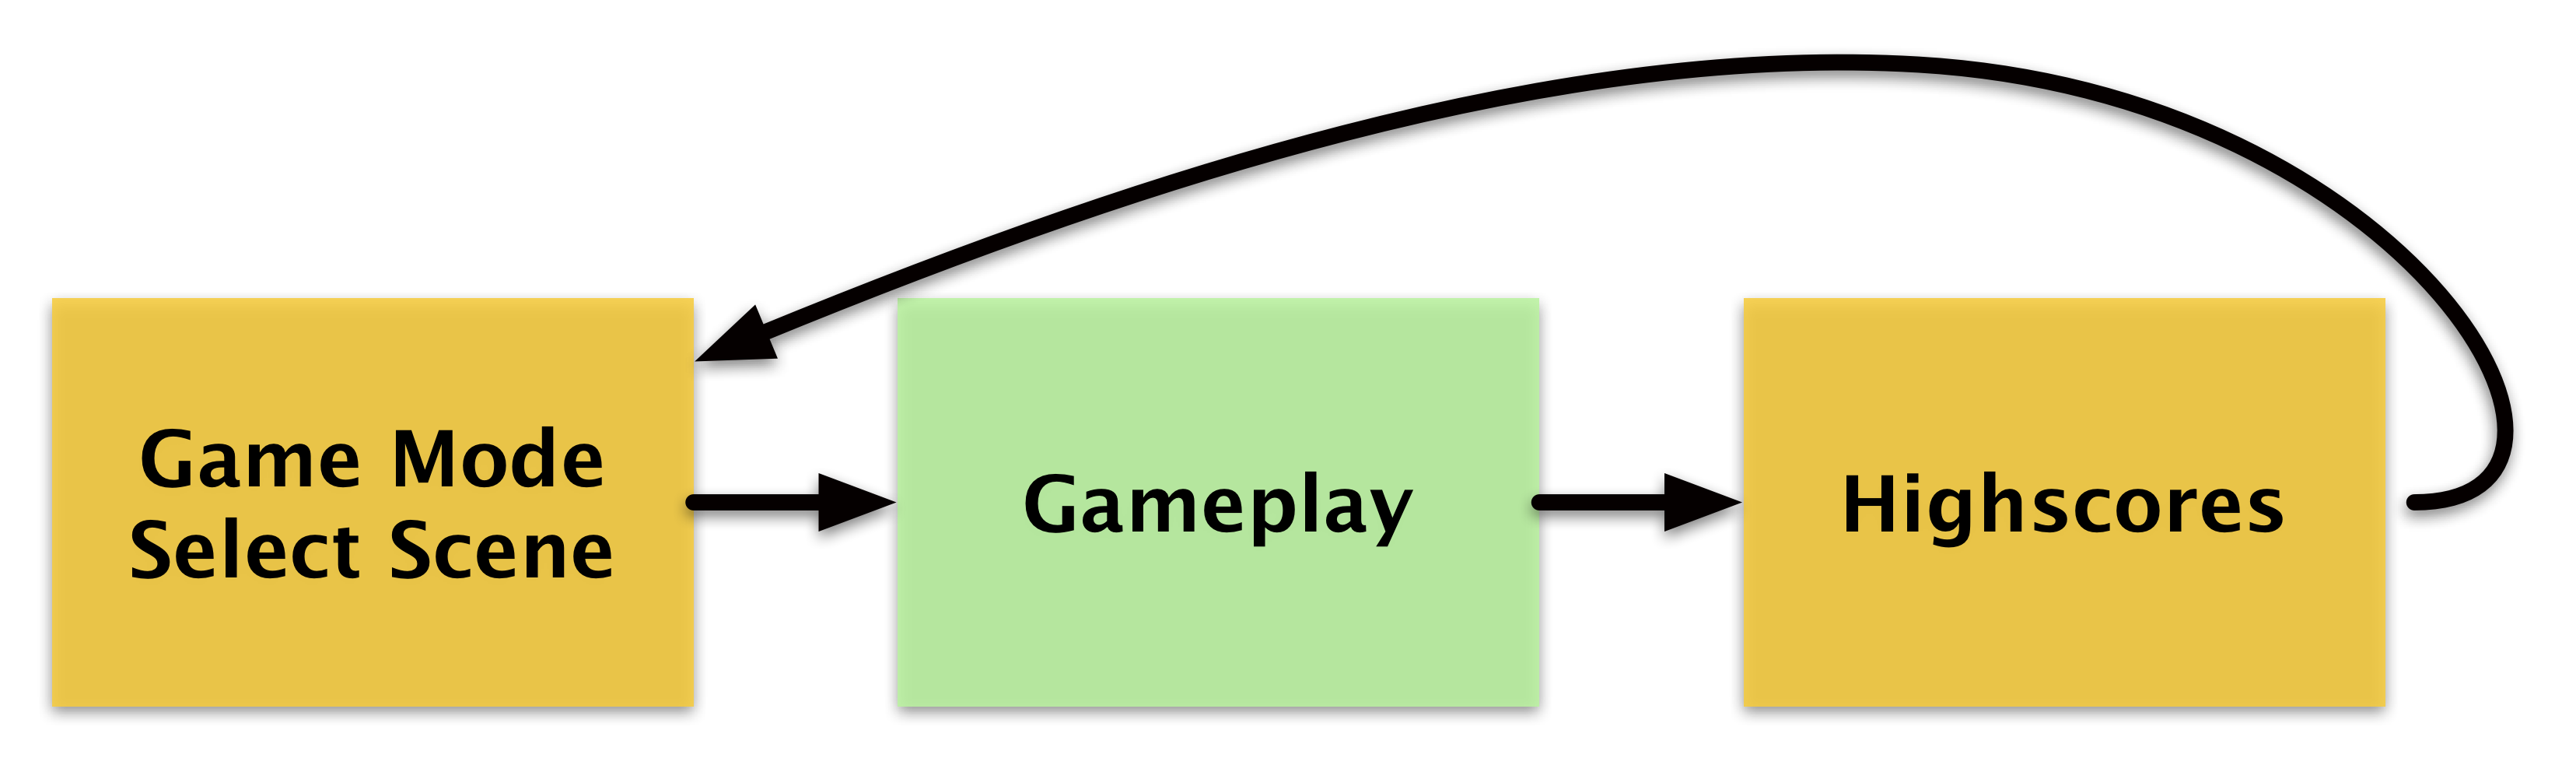
\includegraphics[width=0.7\linewidth]{images/Chapter6/screen_flow.png}
\end{figure}

Throughout this chapter you will not only learn how to build user interfaces
with \cocos{} and \SB{}, you will also learn how to structure this game to
support two different gameplay modes. We will implement and \textit{endless} and
a \textit{timed} gameplay mode, each with a different set of rules and
behaviors.

Let's start out by adding the game mode selection scene!

\section{Adding a game mode selection scene}
We will now change the screen flow of our existing game. Instead of diving into
the gameplay directly the user will see a game mode selection scene when
starting the game. 

The game mode selection scene will allow the user to swipe to switch between the
endless and timed game mode. Luckily \cocos{} provides a component called
\inlinecode{CCScrollView}\index{User Interface!CCScrollView} that implements
most of the functionality that we need for that scene.

\subsection{Setting the up the Start Scene}

\begin{leftbar}
Open the \SB{} project and create a new File (File -> New -> File\ldots). Name
the new file \textit{StartScene} and select \texit{Scene} as the type.
\end{leftbar}

We will create a game mode select scene that smoothly transitions into the
gameplay. To accomplish that we'll use the same background image for this scene
as for the actual gameplay. 

\begin{leftbar}
Drag the image \textit{backround.png} image onto the stage; it becomes the first
child of the root node of our new \textit{StartScene}.
\end{leftbar}

The background image should have exactly the same settings as in
\textit{MainScene} so that it fills the entire scene.

\begin{leftbar}
Select the background sprite in the timeline and apply the following steps:
\begin{enumerate}
  \item Set the position type for X to \textit{percentage of parent container}
  \item Set the X position to \textit{50}
  \item Set the position type for Y to \textit{percentage of parent container}
  \item Set the Y position to \textit{50}
\end{enumerate}
\end{leftbar}

Now the background image should fill the entire background. We will be
presenting some information in front of that background. To make that
information stand out more we will dim the background a little bit by turning
down its opacity. Since the fill color behind the background image is black a
lower opacity will result in a darker image.

\begin{leftbar}
Select the background sprite in the timeline. Set the opacity in the property
inspector to \textit{0.7}:
\begin{figure}[H]
		\centering
		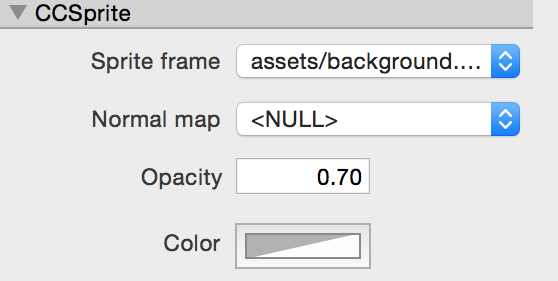
\includegraphics[width=200pt]{images/Chapter6/opacity_lower.png}
\end{figure}
\end{leftbar}

Next, we are going to add a label with an instruction for the player. A label is
a simple UI component that can display text. When building games with \cocos{}
we want to place the most UI components relative to screen edges. Using this
approach the UI will still look good when the game runs on a device with a
different screen size. Here's a little illustration:

\begin{figure}[H]
		\centering
		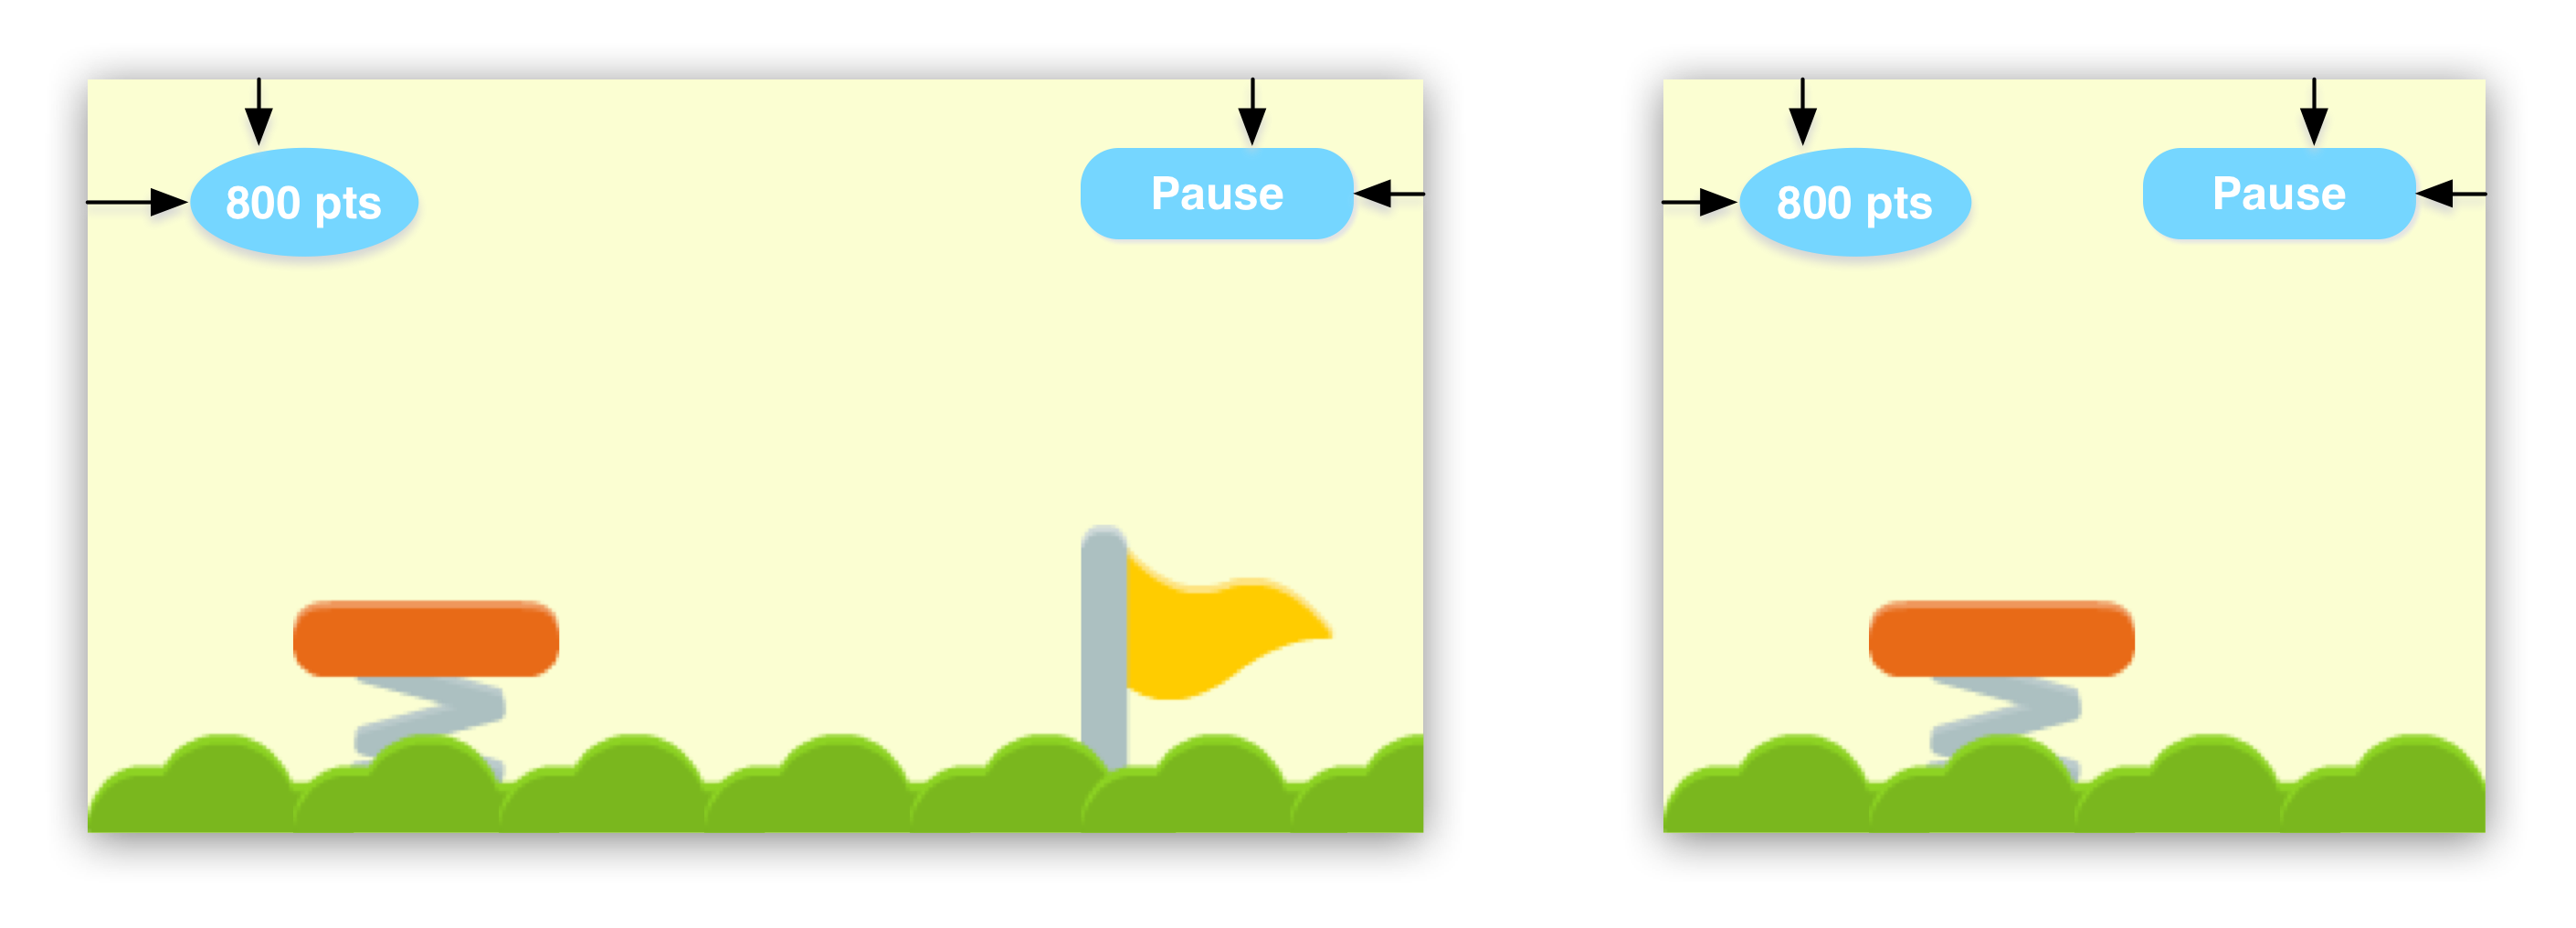
\includegraphics[width=0.7\linewidth]{images/Chapter6/multiple_screen_sizes.png}
		\caption{UI elements should be placed relative to screen edges to preserve
		their position on different screen sizes}
\end{figure}

Throughout this chapter we will use \cocos{}'s reference
corner feature to accomplish resizable user interfaces. 

\begin{leftbar}
Drag a \textit{CCLabelTTF} from the node library \textit{onto} the background
sprite, so that it becomes a child of it. Set the position up as following:
\begin{enumerate}
  \item Set the position to be relative from the \textit{Top-left}.
  \item Set the position type for X to \textit{percentage of parent container}
  \item Set the X position to \textit{50}
  \item Set the Y position to \textit{80}
\end{enumerate}

Set the label text to: \textit{Choose your game mode:}. We also want to change
the font and appearance of this label a little:
\begin{enumerate}
  \item As font name choose: \textit{Optima-Bold}
  \item As font size choose: \textit{40}
  \item Set the draw color to \textit{black}
  \item Set the outline color to \textit{white}
  \item Set the outline width to \textit{6}
\end{enumerate}
\end{leftbar}

After setting the label up your start scene should look as following:

\begin{figure}[H]
		\centering
		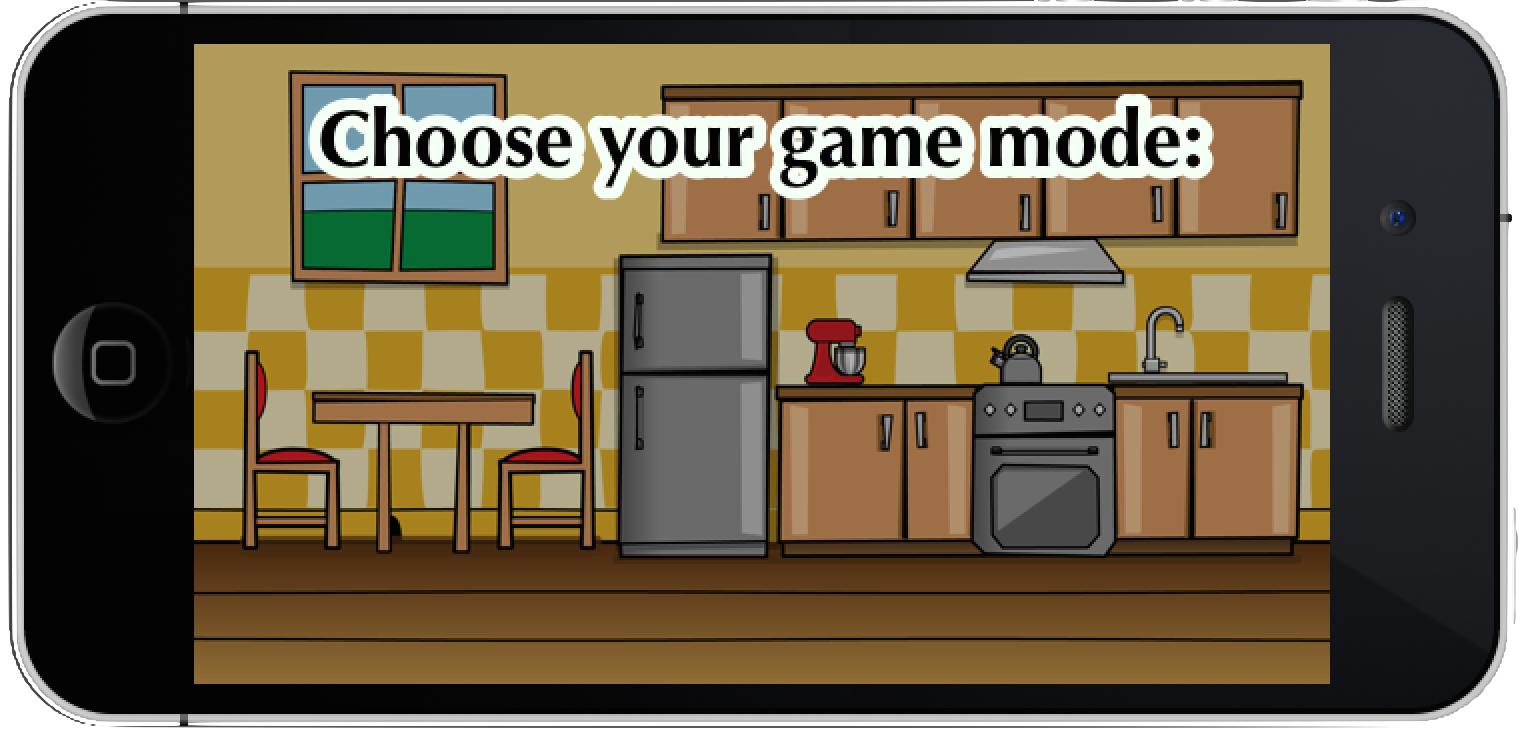
\includegraphics[width=0.7\linewidth]{images/Chapter7/start_scene.png}
		\caption{UI elements should be placed relative to screen edges to preserve
		their position on different screen sizes}
\end{figure}

There's a lot more work left to do! As mentioned earlier we will create a scroll
view that let's the user swipe between two different game modes. Every scroll
view has a content node. That content node is larger than the size of the scroll
view and the scroll view can be used to view different parts of this content
node. Here's an illustration:

\begin{figure}[H]
		\centering
		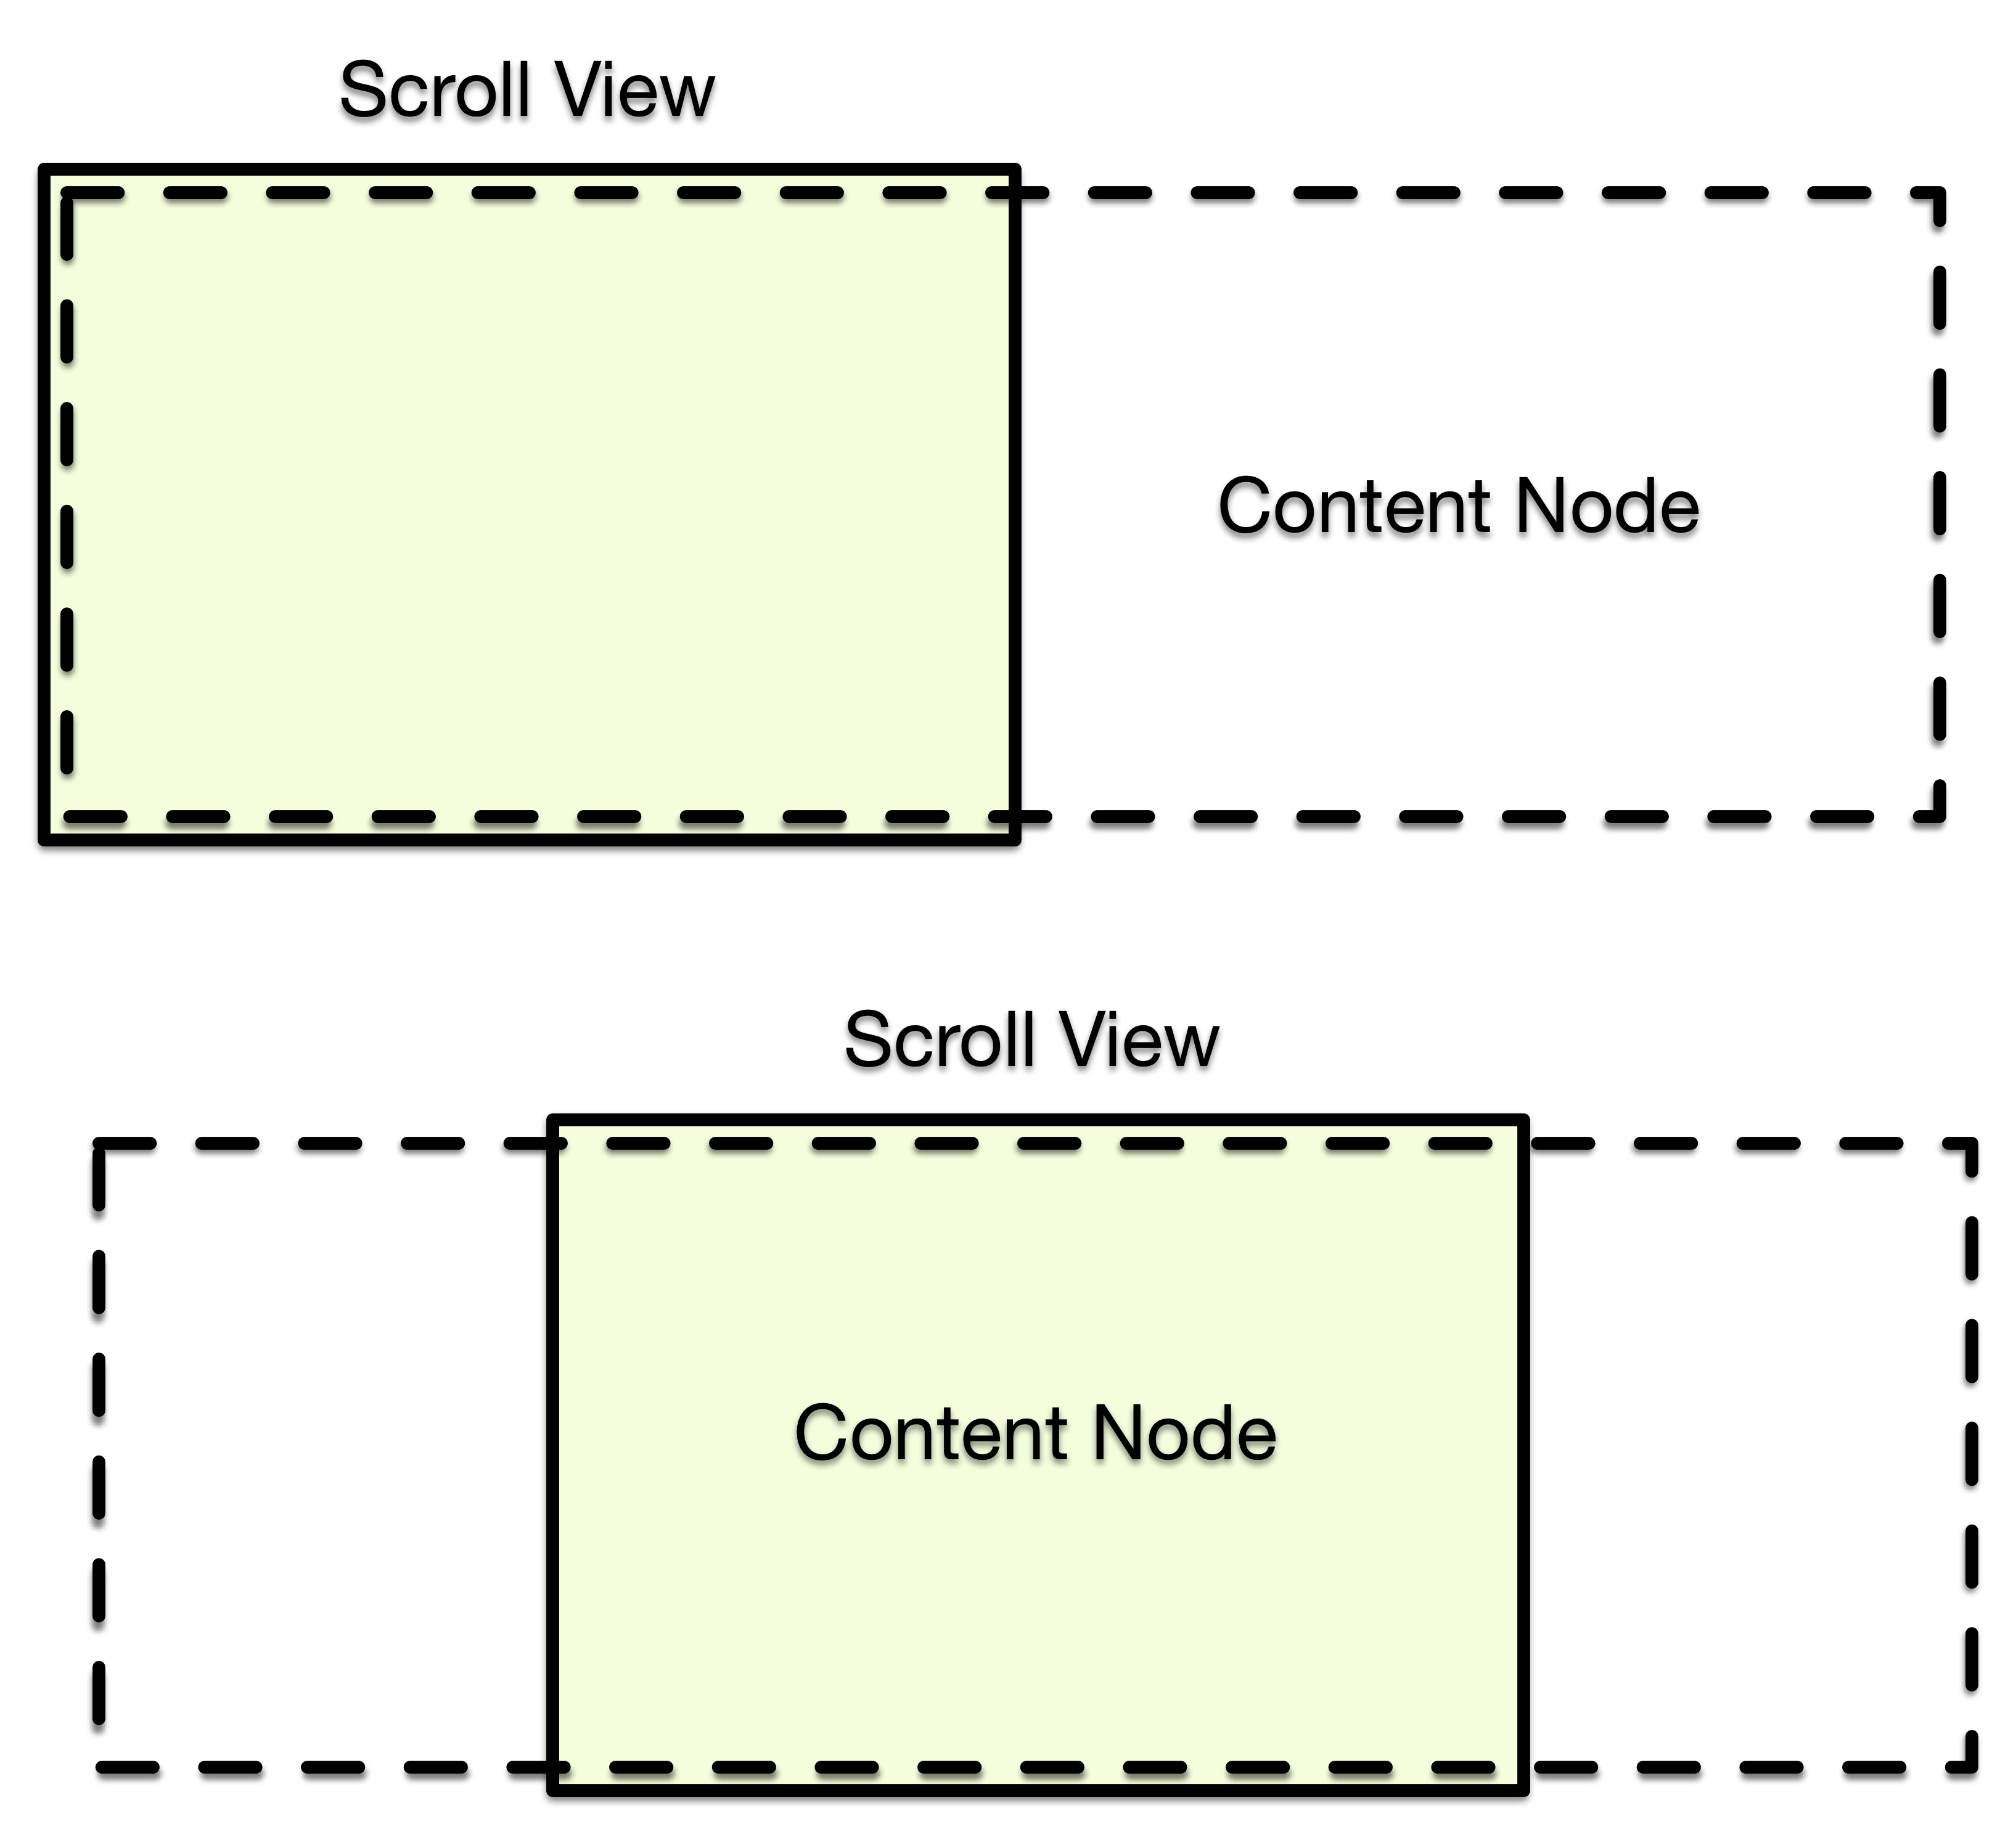
\includegraphics[width=0.5\linewidth]{images/Chapter7/scrollview_concept.png}
		\caption{The scroll view can present different portions of its larger content
		node. The user can change the displayed portion by swiping.}
\end{figure}

Our next step will be creating this content node. In general scroll views allow
users to scroll to any arbitrary position within the scroll view's content node.
In our specific example we would like to change this behavior. We only
want the user to select between two different game modes, each of these game modes will be
represented by a full screen node. It wouldn't make sense to allow the user to
scroll half way between the endless and timed game mode. For this specific case
the scroll view provides an option called \textit{Paging enabled}. If you want
to use a scroll view with paging your content node needs to have a size that is
a multiple of the scroll view's size. In our particular example the content node
for our scroll view will be twice as wide as the scroll view itself, resulting
in a scroll view with two pages. When paging is enabled, the scroll view will
always snap to one of the two pages as soon as a user stops scrolling. If this
sounds a little bit too abstract for you, it should become clearer as we implement and use the scroll view.

\subsection{Creating the content node for the scroll view}

First we need to create the content view. We will set it up in a separate
\ccbfile{} file. 
\begin{leftbar}
Create a new \ccbfile{} called \textit{GameModeSelectLayer} and choose its type
to be a \textit{Layer}.
\end{leftbar}

\begin{details}[frametitle={Why are we using a Layer to create the scroll view
content?}]\index{Document Types}
A short refresher on the different \ccbfile{} types: Scenes are used to
represent full screen content. Sprites are used for simple Sprite Images. Nodes
are used for node compositions that don't have a specific content size. Layers
are used to create content within a stage that has a fixed size.
Layers are typically used for popups or scroll view content nodes because we
want to layout the content based on a container size. We can still use relative
positioning within layers. When the root node of the layer \ccbfile{} gets added
to another node its size will be determined and all relative layouts will be
applied accordingly. We'll use relative positioning for the content node we are
about to create.
\end{details}

\begin{leftbar}
Select the root node of \textit{GameModeSelectLayer.ccb} and choose the width
and height to be in percentage of the parent container. Choose 100\% for the
height and 200\% for the width of the node:
\begin{figure}[H]
		\centering
		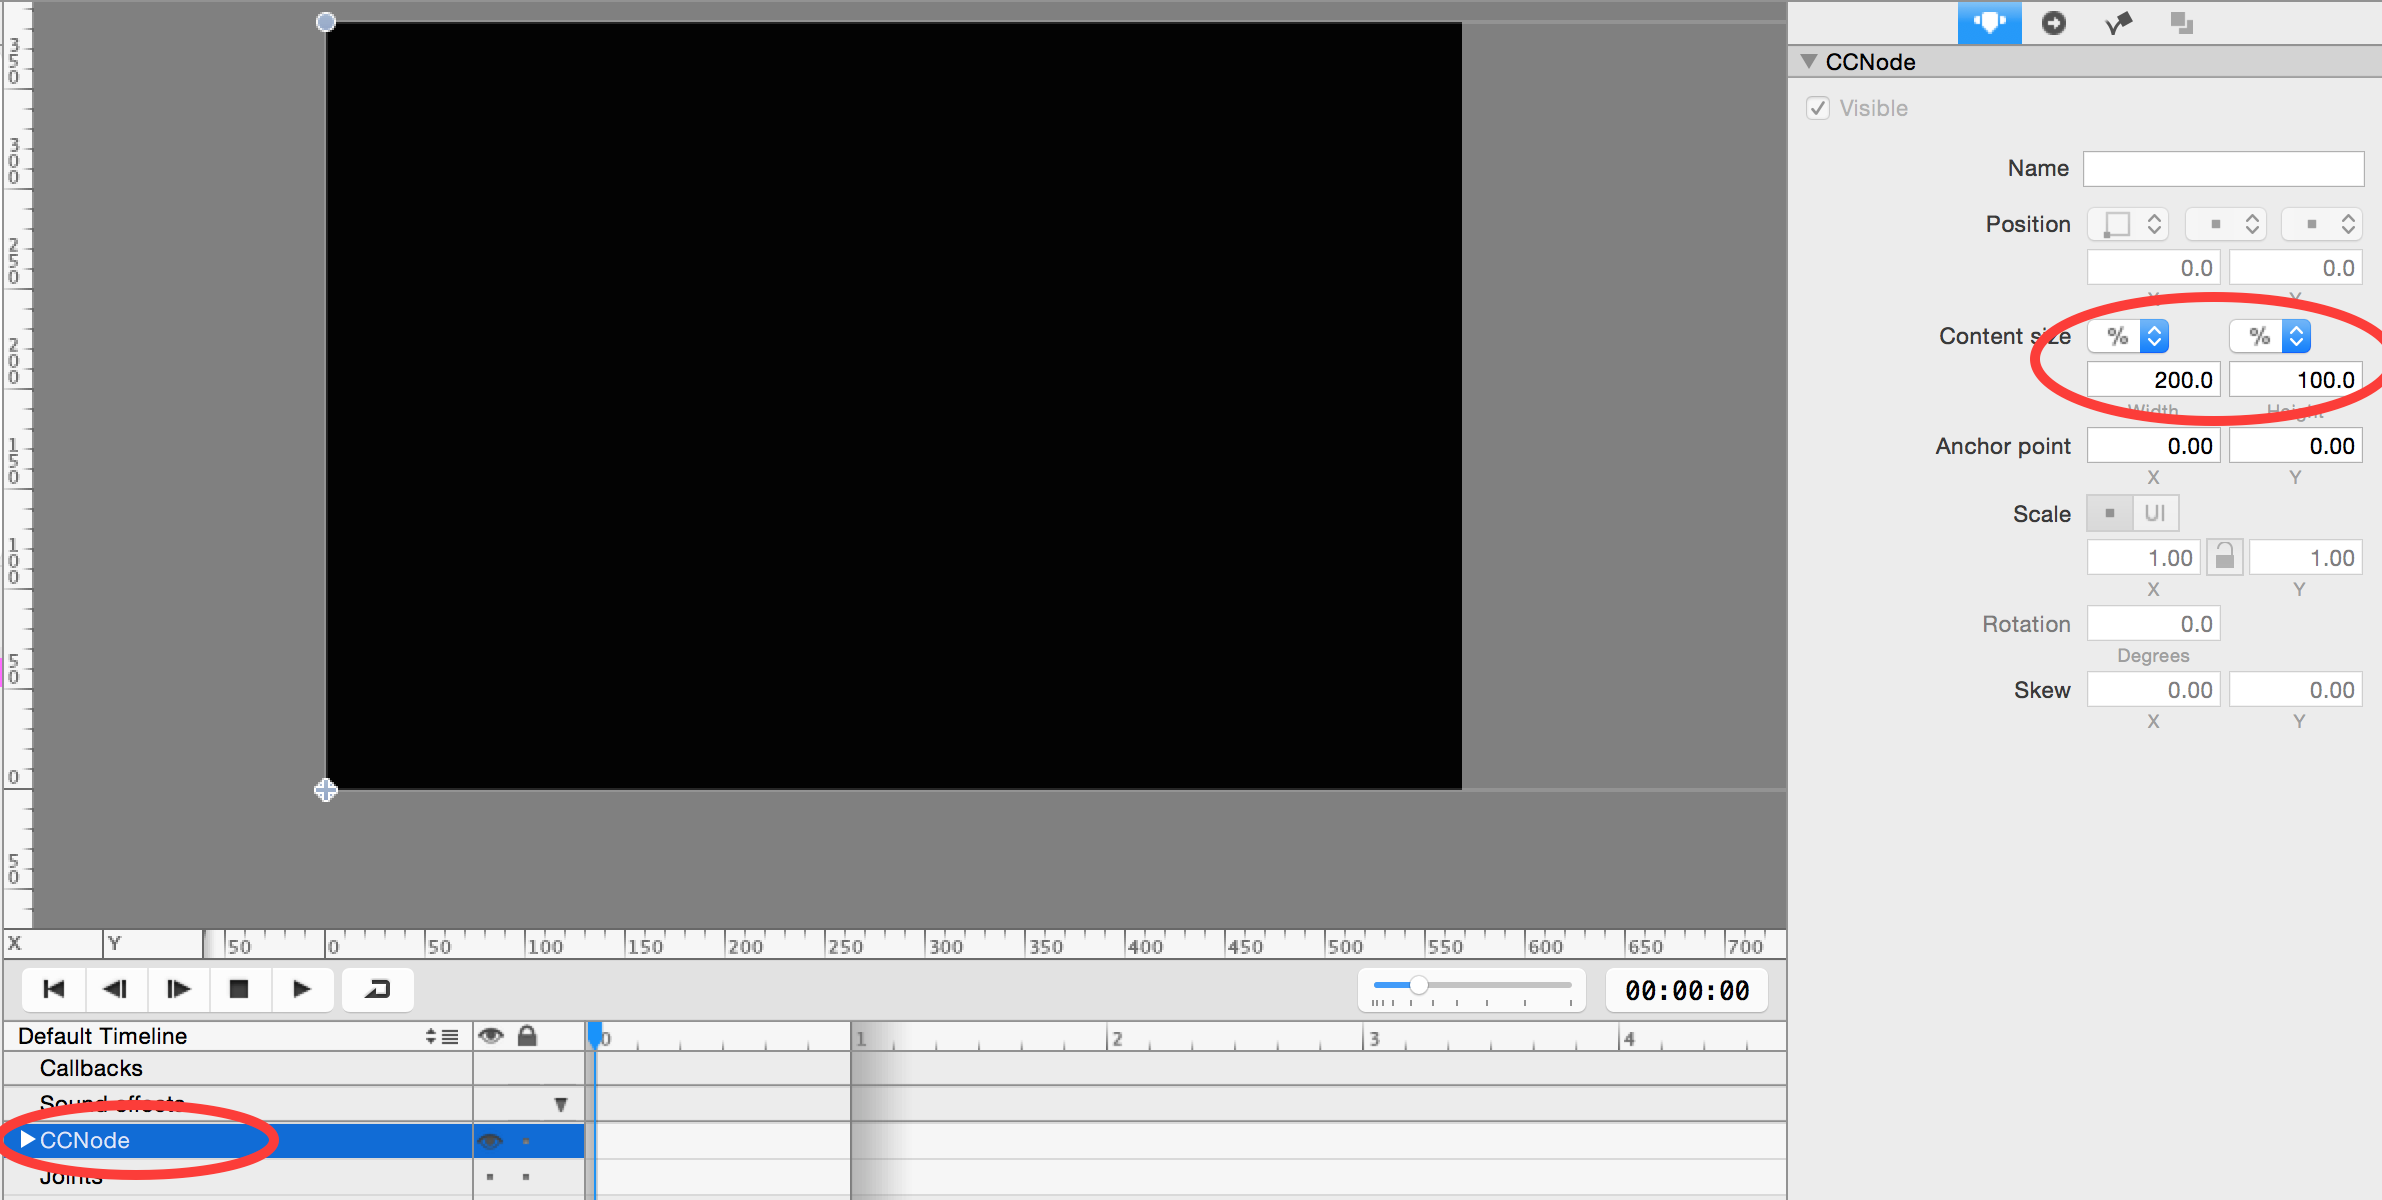
\includegraphics[width=0.6\linewidth]{images/Chapter7/content_node_width.png}
\end{figure}
\end{leftbar}
We want the scroll view to contain two pages, that means the content node needs
to be exactly double as wide as the scroll view. Because we are setting up the
size of the root node of this \ccbfile{} in percentage of the parent container,
its actual size will only be determined when it is added to a scroll view. This
is a great example of dynamic layouts; our scroll view could have any
arbitrary size and this content node would always be exactly twice as wide.

Inside of this root node we are going to place the content for our two different
pages. To provide a clean structure we will create one container node for each
page.

\begin{leftbar}
Add a \ccnode{} as a child to the root node. Name this child
\textit{endless-mode} by selecting the node in the timeline and hitting the
return key. Set the content type of the node to be in percentage of the parent
container. Set the width to 50\% and the height to 100\%. The container for the
left page is set up.
\end{leftbar}

\begin{leftbar}
Add a second \ccnode{} as a child to the root node. Name this child
\textit{timed-mode}. Set the content type of the node to be in percentage of the parent
container. Set the width to 50\% and the height to 100\%. Additionaly, set the x
position to be in percentage of the parent container and set the value to 50\%.
\end{leftbar}

Now we have containers for each page set up. We are going to fill them with
labels that describe the game mode represented on each page and an arrow
indicating that there is another game mode available by swiping across the
screen. This is what the completed content node will look like:

\begin{figure}[H]
		\centering
		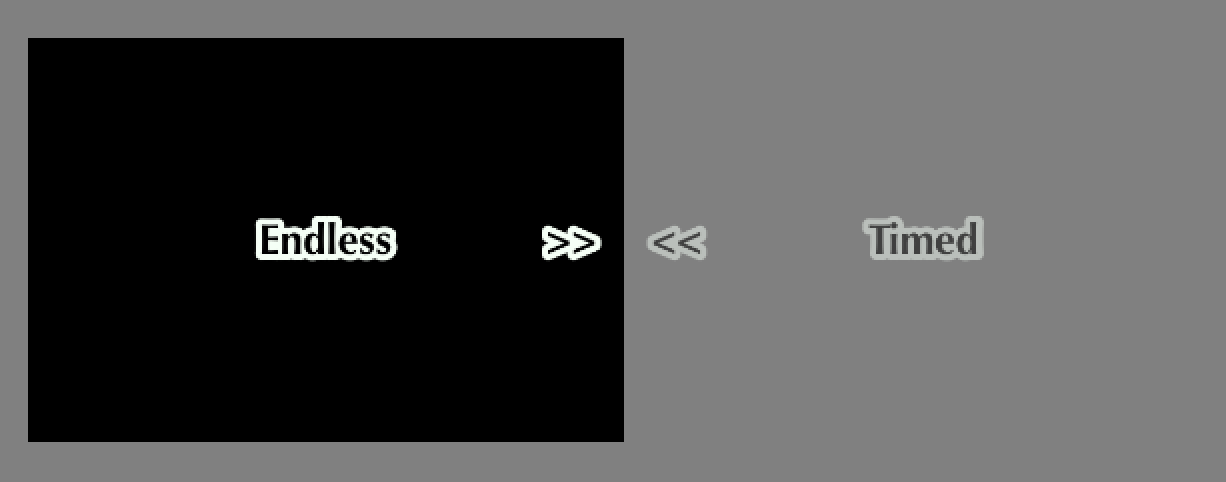
\includegraphics[width=0.6\linewidth]{images/Chapter7/content_node_completed.png}
		\caption{The completed content node by the end of this section.}
\end{figure}

First, let's add the labels for the endless mode.

\begin{leftbar}
Drag a \cclabel{} from the node library onto the \textit{endless-mode} node.
Center the label within its parent node by choosing a position type of
percentage of parent container. Then set x and y position to 50\%. This label
should look the same as the \textit{Choose your game mode} label on the start
scene. Apply the following settings:
\begin{enumerate}
  \item Set the label text to \textit{Endless}
  \item As font name choose: \textit{Optima-Bold}
  \item As font size choose: \textit{40}
  \item Set the draw color to \textit{black}
  \item Set the outline color to \textit{white}
  \item Set the outline width to \textit{6}
\end{enumerate}
\end{leftbar}

Next, let's add the arrow on the right side that will indicate that the player
can switch to the timed game mode.

\begin{leftbar}
Drag a \cclabel{} from the node library onto the \textit{endless-mode} node.
Apply the following settings:
\begin{enumerate}
  \item Set the label text to \textit{>>}
  \item As font name choose: \textit{Optima-Bold}
  \item As font size choose: \textit{40}
  \item Set the draw color to \textit{black}
  \item Set the outline color to \textit{white}
  \item Set the outline width to \textit{6}
  \item Set the position up as following: \begin{figure}[H]
										  \centering
										  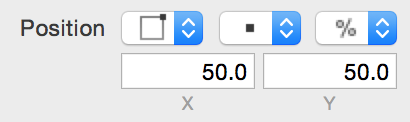
\includegraphics[width=150pt]{images/Chapter7/arrow_label_position.png}
										  \end{figure}
\end{enumerate}
\end{leftbar}

Now your stage should look like this:
\begin{figure}[H]
\centering
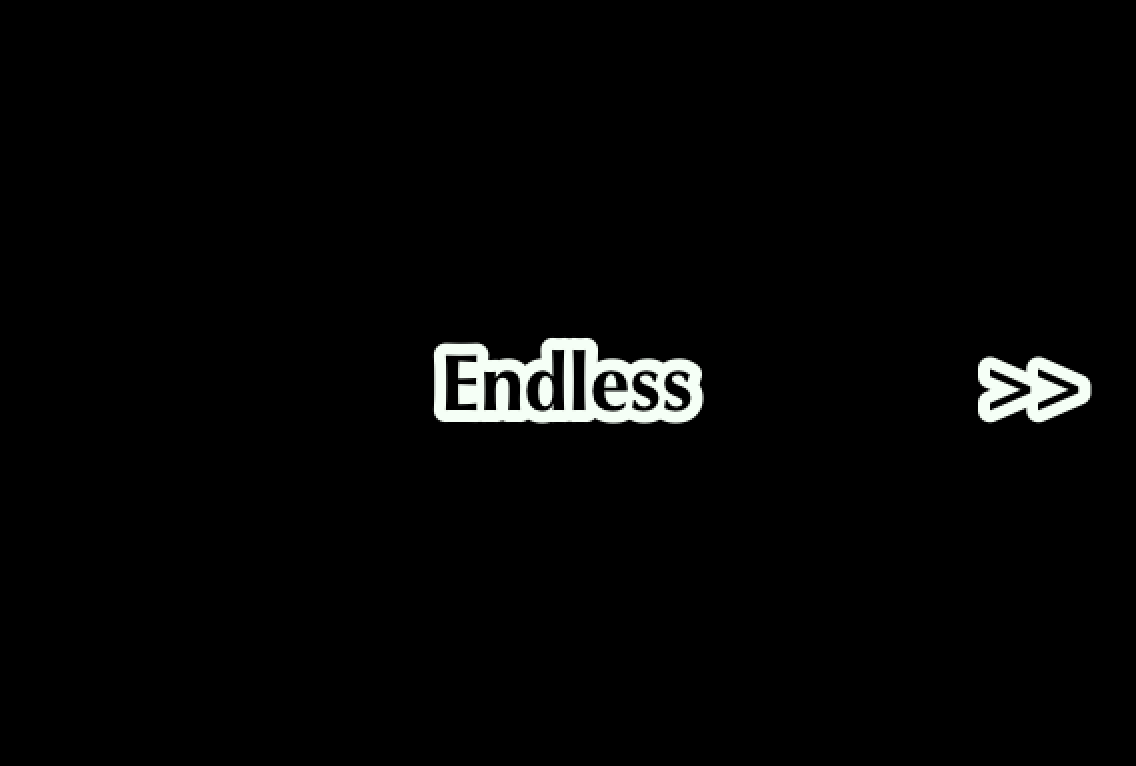
\includegraphics[width=150pt]{images/Chapter7/endless_mode.png}
\end{figure}
We're going to add a little visual detail to this game mode selection layer. The
arrows indicating the other available shall blink. This can be easily
accomplished using \SB{}'s timeline feature. 

\begin{leftbar}
Set the timeline duration to 1 second:
\begin{figure}[H]
\centering
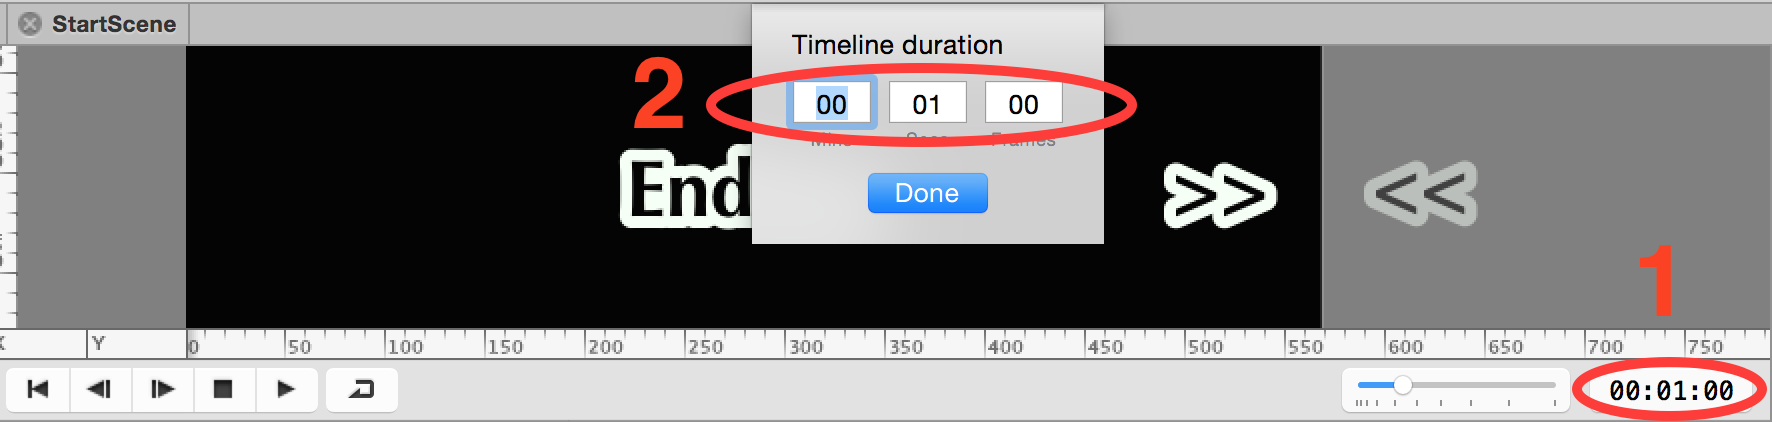
\includegraphics[width=300pt]{images/Chapter7/timeline_duration.png}
\caption{Changing the timeline duration}\label{fig:
timeline_duration}\index{SpriteBuilder Timeline!Change Duration}
\end{figure}
\end{leftbar}

Now we are going to use three \textit{opacity} keyframes to create the blinking
animation. 
\begin{leftbar}
Select the label with the arrows in the timeline. Then create three
keyframes by hitting the \textit{O} (like in opacity) key on your keyboard.
Alternatively you can create keyframes through the top bar menu:
\textit{Animation -> Insert Keyframe\ldots -> Opacity}. Place the first keyframe
at 0 seconds the second one at 0.5 seconds and the third one at 1
second.
\end{leftbar}

Now we can set different opacity values for each of these keyframes and \SB{}
will create smooth animations between them. There are two ways to set a
specific value for a keyframe. You can select the keyframe and change the
relevant property in the property inspector in the right panel of \SB{}. The
easier way however is to double-click onto a keyframe. That will bring up a
small popup in which you can modify the relevant values:
\begin{figure}[H]
\centering
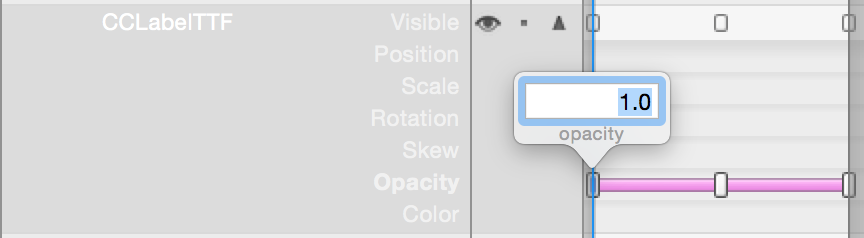
\includegraphics[width=250pt]{images/Chapter7/edit_keyframe.png}
\caption{Double-click onto keyframes to modify their values}
\end{figure}

\begin{leftbar}
Set the opacity in the first keyframe to 0. Set the opacity to 1 in the second
keyframe. For the third keyframe set the opacity to 1 again.
\end{leftbar}

Now the arrow will appear for half a second and then disappear for another half
a second. We don't want this animation to be over after 1 second. Instead we
want to loop it forever. We can do so by \textit{chaining}\index{\SB{}
Timeline!Chaining} the timeline to itself. In \SB{} timelines can be chained to
each other. That means that you can define that another timeline should run
after the current timeline is completed. If you use this feature to chain a
timeline to itself you have an endlessly running timeline animation!

\begin{leftbar}
Chain the default timeline to itself as shown below:
\begin{figure}[H]
\centering
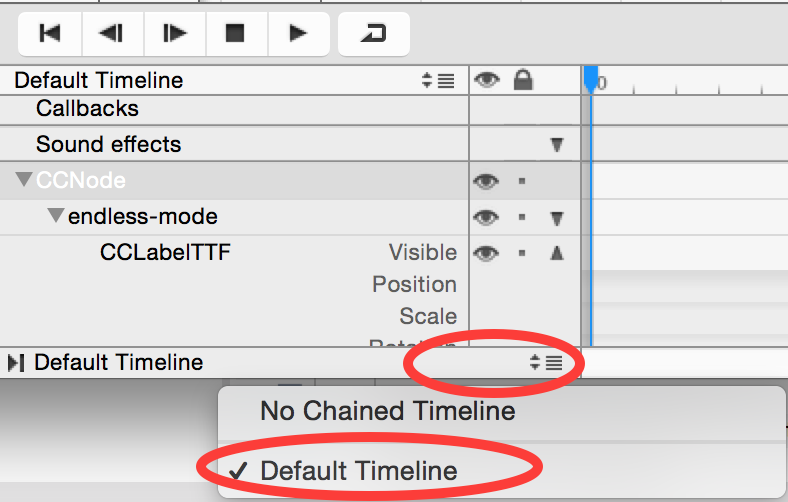
\includegraphics[width=200pt]{images/Chapter7/chain_timeline.png}
\caption{Double-click onto keyframes to modify their values}
\end{figure}
\end{leftbar}

\begin{details}[frametitle={Looping animations in \SB{}}]
Animations that are set up with a chained timeline will loop endlessly when your
game is running on a simulator or phone. In \SB{} itself the animation will only
run once. If you want to preview what your animation will look like when it is
looped, you need to use the following control in the timeline playback panel:
\begin{figure}[H]
\centering

\includegraphics[width=100pt]{images/Chapter7/loop_timeline.png}
\end{figure}
Note that this control will only affect your previewed animation in \SB{}. Not
the actual animation running in your game.
\end{details}

Now we are finished setting up one of the two game modes. Setting up the node
for the timed game mode involves exactly the same steps as you have seen just
now. The only difference is the arrow label. The arrows should be pointing to
the left and the arrow should be positioned from the left edge of the
\textit{timed-mode} node. I will leave this as an exercise to you. Remember that
you can always check the solution on GitHub if you get stuck. Once you have set
up the node for the second game mode come back and we'll integrate this game
mode selection layer into the start scene.

\begin{leftbar}
Switch to the \textit{StartScene.ccb} file and drag a \textit{CCScrollView} from
the node library onto the \textit{background} node. Set the position to 0,0. The
scroll view shall cover the entire screen, so set the size type to
\textit{percentage of parent container} and choose 100\% for the width and the
height of the scroll view. Set up the scroll view specific settings in the
property inspector as follows:
\begin{figure}[H]
\centering
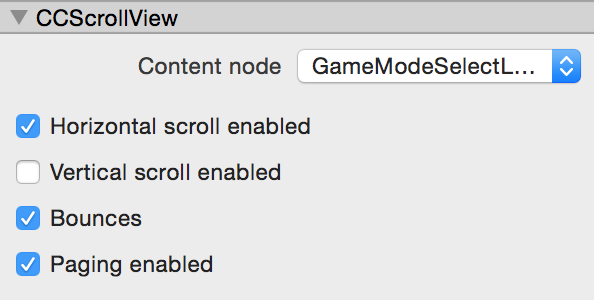
\includegraphics[width=250pt]{images/Chapter7/scrollview_settings.png}
\end{figure}
\end{leftbar}
Let's discuss the scroll view settings briefly. The most important property is
the \textit{Content node} property. Here you can choose a \ccbfile{} that will
be displayed inside of the scroll view. We choose the
\inlinecode{GameModeSelectLayer.cbb} that we just created. We check
\textit{Horizontal scroll enabled} because the user shall only be able to scroll
left and right, not up or down. We discussed the option \textit{paging enabled}
briefly at the beginning of this section. With this setting activated the scroll
view will always snap to one of the game modes and will not allow the user to
stop scrolling in the middle of two game modes.

Great! At this point the set up of our start scene is almost complete.

\subsection{Finishing up the game mode selection scene}
As a last step we will implement the actual selection of one of the two game
modes. So far we have a scroll view that will allow users to switch between the
game modes but we don't have a mechanism to select one of the two and start a
game.

We will add a \textit{start} button to \textit{StartScene.ccb} that will
allow users to confirm a selected game mode and start the game. Once we have the button set up we will
add an animated transition from this game mode selection screen to the gameplay
scene. That transition will be triggered as soon as the player taps the start
button.

Let's start by adding a plain button. It is going to be positioned towards
the bottom of the screen, below the label that shows the selected game mode.

\begin{leftbar}
Open \textit{StartScene.ccb} and drag a \textit{Button} from the node library to
the stage, make sure it is a child of the \textit{background} node.
Set the button up as following:
\begin{enumerate}
  \item Set the \textit{Position Reference Corner} to \textit{Bottom-left}
  \item Set the x position to be \textit{In percent of parent container}
  \item Set the x position to \textit{50} to center the node
  \item Set the y position to \textit{80}
  \item Set the \textit{Preferred size} to \textit{100.0, 40.0}
  \item Set the \textit{title} to \textit{Start!}
  \item Set the \textit{Font name} to \textit{Optima-Bold}
  \item Set the \textit{Font size} to \textit{17.00} 
\end{enumerate}
\end{leftbar}

Let's discuss some of these properties we just set up. As a short reminder - in
almost all cases we want to position UI elements relative to the screen corner
which they are closest to. This will result in the best behavior when the game
runs on different screen sizes. Therefore we choose the \textit{Bottom-Left}
corner as reference corner (technically we could also choose the
\textit{Bottom-Right}, since we are centering the button horizontally this
wouldn't make any difference).

Another interesting property is the \textit{Preferred Size}. Buttons
automatically resize to be large enough surround their content (in this case
the button text). If we want a button to appear larger than necessary we can set
the \textit{Preferred Size} property. In this example we make the button a
little bit larger than required to fit the text \textit{Start!}.

We also need to set up some code connections. When the user taps the button we
want to start the transition. And there's another little feature that's
important. We only want to activate the \textit{Start!} button when the user has
selected one of the two game modes. If the user is currently scrolling between
two screen modes it shouldn't be possible to start the game. Otherwise it could
be pretty unclear to the user which game mode has been selected. We're going to
solve this issue by deactivating the button when a user is scrolling between
game modes.

\begin{leftbar}
Select the \textit{Start!} button and open the \textit{Code Connections}
tab. Set up a code connection with the \textit{Doc root var} and call it
\textit{playButton}. 
\end{leftbar}

We are going to use this code connection to active and deactivate the start
button. Towards the beginning of this book we have discussed how we can connect
method calls to button taps (\ref{target_selector}). Now we are going to use
this functionality for the start button.

\begin{leftbar}
Set the \textit{selector} (method name) to \textit{playButtonPressed} and choose
the \textit{target} to be \textit{Document root}.
\end{leftbar}

As soon as the button is clicked the \inlinecode{playButtonPressed} will be
called on the class of the root node. Right now the root node has no class set
up. Let's change that.

\begin{leftbar}
Select the root node (top most node in the timeline) of \textit{StartScene.ccb},
then open the code connections tab. Inside of the code connections tab set the
\textit{Custom class} to \textit{StartScene}.
\end{leftbar}

We'll need one more code connection for this scene - a connection for the
scroll view. Later, when we add some code to this scene you will see that we
need to connect to the scroll view to be informed when the scroll view
starts/stops scrolling. Whenever that happens we need to deactivate and activate
the start button accordingly.

\begin{leftbar}
Select the scroll view from the timeline and open the code connection tab. Set
up a code connection to \textit{Doc root var} and name that connection
\textit{scrollView}.
\end{leftbar}

Now we have all the code connections set up. Before we add some code to make
this scene work we will work through one last step in SpriteBuilder - creating a
nicely animated transition from the selection scene to the gameplay scene.

\subsection{Adding a fancy transition animation}

This is what our transition shall look like:

\begin{figure}[H]
		\centering
		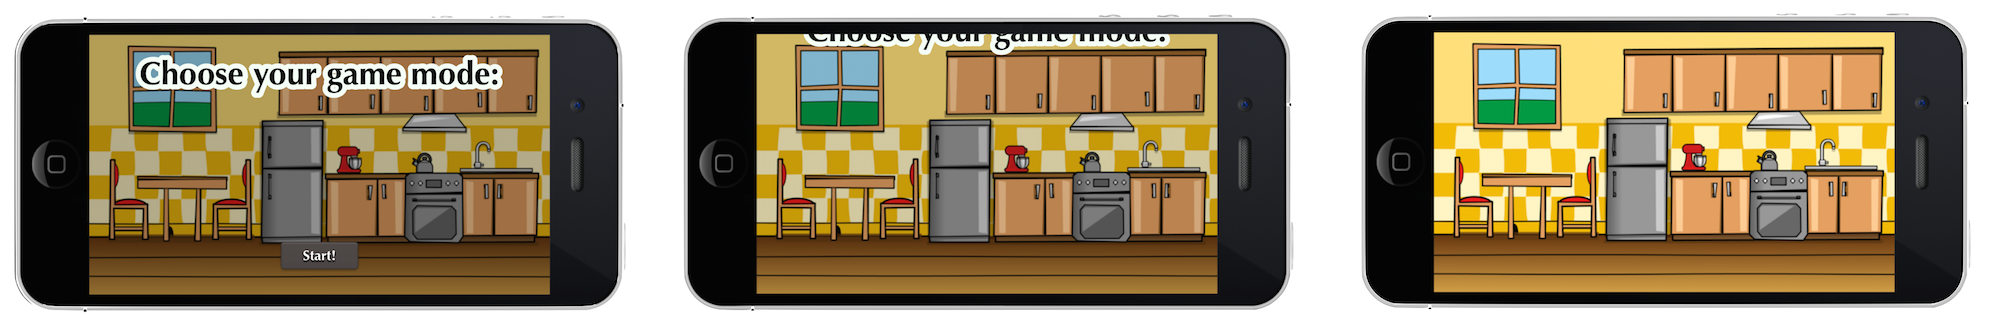
\includegraphics[width=0.85\linewidth]{images/Chapter7/gameplay_transition.png}
		\caption{By moving UI elements out of the screen and brightening the scene up
		we transition from the start scene to the gameplay scene}
\end{figure}

This transition is a nice example of how menus can be integrated into games
seamlessly. Luckily creating this animation is pretty straightforward, using
SpriteBuilder's timeline. There are a bunch of steps involved, but none of them
are complicated. First, we'll need to create a new timeline. The default
timeline runs automatically as soon as the scene becomes visible - the animation
we are about to build, in contrast, shall only run when the user has selected a
game mode. Therefore we need to create new timeline which we can run when
triggered in code.

\begin{leftbar}
Create a new timeline for our transition animation:
\begin{figure}[H]
		\centering
		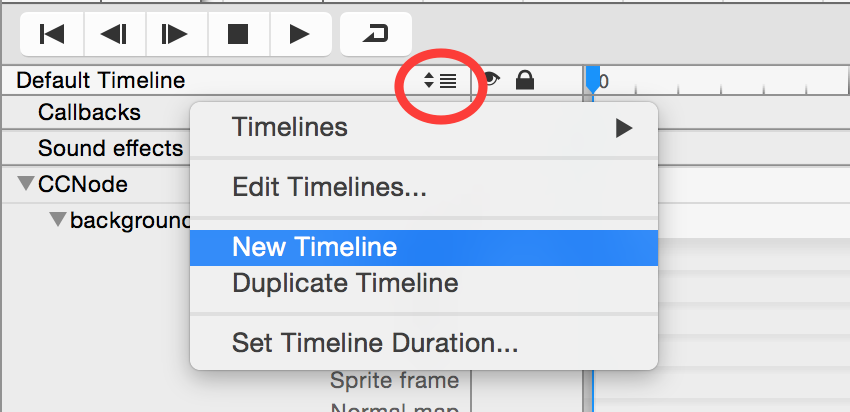
\includegraphics[width=200pt]{images/Chapter7/new_timeline.png}
\end{figure}
Next, rename the timeline. You can access the timeline editor through \SB{}'s
menu (\textit{Animation -> Edit Timelines\ldots}). Change the timeline name to
\textit{StartGameplay}.
\end{leftbar}
We want the transition to be pretty fast, so let's set the timeline duration to
1 second.
\begin{leftbar}
Set timeline duration to 1s. If you forgot how to change the timeline duration
you can skim back a few pages to figure \ref{fig: timeline_duration}.
\end{leftbar}
Next, we are going to set up keyframes for all of the UI elements that we want
to move off the screen. Additionally we will fade in the background sprite. Make
sure to follow the instructions exactly!
\begin{leftbar}
\begin{enumerate}
  \item Select the \textit{background} sprite
  \item Create an \textit{Opacity Keyframe} at 0 seconds and set the opacity
  value to \textit{0.7}
  \item Create a second \textit{Opacity Keyframe} at 1 second and set the
  opacity to \textit{1.0}
  \item Select the \textit{CCButton}
  \item Create a \textit{Position Keyframe} at 0 seconds, leave the position
  unchanged
  \item Create a second \textit{Position Keyframe} at 1 second and set the
  position to \textit{(50\%, -400 points)}
  \item Select the \textit{CCScrollView}
  \item Create a \textit{Position Keyframe} at 0 seconds, leave the position
  unchanged
  \item Create a second \textit{Position Keyframe} at 1 second and set the
  position to \textit{(0, -400)} 
  \item Select the \textit{CCLabelTTF}
  \item Create a \textit{Position Keyframe} at 0 seconds, leave the position
  unchanged
  \item Create a second \textit{Position Keyframe} at 1 second and set the
  position to \textit{(50\%, -50 points)}  
\end{enumerate}
\end{leftbar}
Great! If you want you can test the animation with the \SB{} timeline playback
feature.

There's one last step left in \SB{} before we move to \xcode{} and implement the
actual transition between start scene and gameplay. As soon as the animation
completes, that means all UI elements have moved off the screen and the
background is brightened up completely, we want to switch to the gameplay scene.
Switching scenes has to be implemented in code. This means that we need a
callback in code that gets triggered as soon as this animation completes.

\SB{} and \cocos{} provide three different ways to implement this:
\begin{itemize}
  \item Provide a completion block to the animation manager of a scene. This
  completion block will be called whenever a timeline animation completes
  (\inlinecode{setCompletedAnimationCallbackBlock:})
  \item Implement a delegate method that gets called by the animation manager
  when a timeline animation completes
  (\inlinecode{completedAnimationSequenceNamed:})
  \item Set up a callback method within a \SB{} timeline animation
\end{itemize}

For this section I want to go with the last option. The ability to call methods
as part of timeline animations can be useful in many situations, so I want to
use it as early as possible!

\begin{leftbar}
To add a callback method to a timeline animation you need to \textit{Option-Key
+ Click} into the \textit{Callbacks} line of the timeline editor:

\begin{figure}[H]
		\centering
		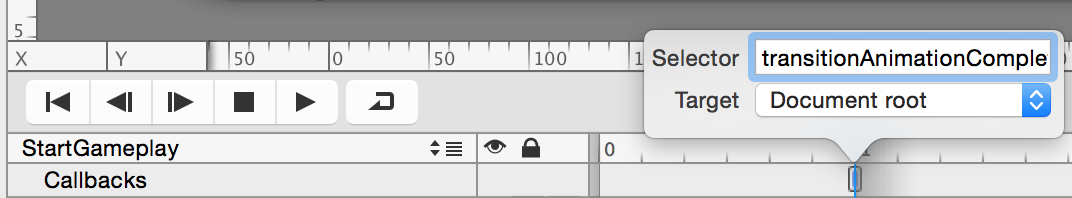
\includegraphics[width=300pt]{images/Chapter7/timeline_callback.png}
\end{figure}
Place that callback at 1 second. You can also choose the \textit{target} and
\textit{selector} for this callback. Select \textit{Document root} as target and
\textit{transitionAnimationComplete} as selector.
\end{leftbar}

Great! This was quite a lot of work, but now we have a game mode selection
scene (including a scroll view) and a great transition into the gameplay scene.
Now it's time to switch back to code and implement the scene transition.

\subsection{Implementing the game mode selection}

\begin{leftbar}
Publish the \SB{} project and switch to the \xcode{} project.
\end{leftbar}

The first change we need to make to the \xcode{} project, is setting up which
scene gets presented when our game starts\index{Start Scene}. By default it's
the \textit{MainScene}. However, we have created a new \textit{StartScene} and want
that one to be the first scene of the game.

We can change this setting in the \textit{AppDelegate} of the project. 
\begin{leftbar}
Open \textit{AppDelegate.m} in \textit{Source/Platforms/iOS/}:
\begin{figure}[H]
		\centering
		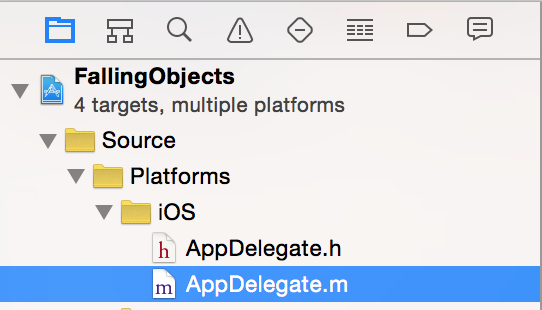
\includegraphics[width=200pt]{images/Chapter7/app_delegate.png}
\end{figure}
\end{leftbar}

The \inlinecode{AppDelegate} of \cocos{} is written in Objective-C. If you don't
know Objective-C, don't worry, the change we need to make is trivial.

When a \cocos{} game starts, the \inlinecode{startScene} method of the
\inlinecode{AppDelegate} gets called. That method is responsible for loading and
returning the start scene of the game. Let's modify it to load
\inlinecode{StartScene} instead of \inlinecode{MainScene}.

\begin{leftbar}
Modify the \inlinecode{startScene} method of \textit{AppDelegate.m} to look as
following:
\begin{lstlisting}
- (CCScene*) startScene
{
    return [CCBReader loadAsScene:@"StartScene"];
}
\end{lstlisting}
\end{leftbar}
Great! Now our new start scene will be presented when our game starts. Note
that the game won't run at this point. We need to create the
\inlinecode{StartScene} class. We're already referencing this class from the
\SB{} project, but we haven't created it yet.

\begin{leftbar}
Create a new Swift file. Call it \inlinecode{StartScene}. Set up the basic
\inlinecode{StartScene} class like this:
\begin{lstlisting}
class StartScene: CCNode {
  
  weak var scrollView: CCScrollView!
  weak var playButton: CCButton!
  var selectedGameMode: MainScene.GameMode = .Endless
  
}
\end{lstlisting}
\end{leftbar}
The first two variables are necessary for the code connections that we set up
in our \SB{} project. The third variable stores which game mode the player has
currently selected. Since the game mode is a choice between multiple options, an
enum is a great way to model this. The enum referenced here
(\inlinecode{MainScene.GameMode}) does not exist yet. We need to add it to the
\inlinecode{MainScene} class.

\begin{leftbar}
Open \textit{MainScene.swift} and add the following lines:
\begin{lstlisting}
var gameMode:GameMode?
  
enum GameMode: Int {
  case Endless
  case Timed
 }
\end{lstlisting}
\end{leftbar}
The first line is a property that stores the game mode of the current game.
Later we will use that property to apply different rules to the gameplay and
display different score information. Once the user has selected a game mode, the
\inlinecode{StartScene} will set this property on the \inlinecode{MainScene}.

We've also added an enum definition. The \inlinecode{GameMode} enum has two
different states, one for each game mode. For now we will only implement an
endless and a timed game mode. As we've done earlier, we are associating
\textit{raw values} with this enum by adding the \inlinecode{Int} type after the
enum name. This means that the \inlinecode{Endless} value corresponds to 0 and
the \inlinecode{Timed} value corresponds to 1.

Now we can switch back to working on our new start scene. There are three
features we need to implement in \textit{StartScene.swift}. We need to keep
track of the movement of the scroll view. When the user scrolls to one of the
two pages of the scroll view, we need to remember which game mode has been
chosen. Further, as discussed earlier, we need to deactivate the \textit{Start!}
button while the user scrolls. Finally, we need to trigger a transition to the
gameplay scene (\inlinecode{MainScene}) as soon as a user taps the start button.
As part of that transition we need to inform \inlinecode{MainScene} which game
mode was selected. Let's start with the scroll view related code.

\subsubsection{Implementing a scroll view delegate}\index{User
Interface!CCScrollView!Delegate}
If you have written code for the iOS platform before, you are very familiar with
the principle of delegation. Since this book does not necessarily require
previous iOS app development knowledge, I will give you a brief introduction.

Delegation is often used in iOS frameworks when an object A wants to provide an
object B with the ability to modify object A's behavior or to listen to changes
of object A. However, object A does not need to know the exact type of object B.
Instead, all of the methods that object B can implement are described in a
protocol. Any object can implement this protocol and be the \textit{delegate} of
object A.

\begin{details}[frametitle={Delegate pattern}]
Delegation is used so frequently as part of iOS development that Apple has a
short chapter about it in it's documentation:
\url{https://developer.apple.com/library/ios/documentation/General/Conceptual/DevPedia-CocoaCore/Delegation.html}
\end{details}

The \inlinecode{CCScrollView} in \cocos{} also uses the delegate pattern. This
is what the (Objective-C) protocol looks like:
\begin{lstlisting}
@protocol CCScrollViewDelegate <NSObject>

@optional
- (void)scrollViewDidScroll:(CCScrollView *)scrollView;
- (void)scrollViewWillBeginDragging:(CCScrollView *)scrollView;
- (void)scrollViewDidEndDragging:(CCScrollView * )scrollView willDecelerate:(BOOL)decelerate;
- (void)scrollViewWillBeginDecelerating:(CCScrollView *)scrollView;
- (void)scrollViewDidEndDecelerating:(CCScrollView *)scrollView;

@end
\end{lstlisting}

There are a total of five methods that we can implement. The optional keyword
marks a section of the protocol in which all listed methods are not required to
be implemented. In this specific protocol \textit{all} methods are optional. We
want to be informed when the scroll view starts and ends scrolling. There are
two methods that get called in these cases:
\inlinecode{scrollViewWillBeginDragging} and
\inlinecode{scrollViewDidEndDecelerating}. Let's implement these methods and
become the delegate of our scroll view.

The first step, is setting ourselves up as the delegate of the scroll view. We
can set ourselves as the delegate as soon as the scene is entirely loaded (when
\inlinecode{didLoadFromCCB} is called). 
\begin{leftbar}
Add the following implementation of \inlinecode{didLoadFromCCB} to
\inlinecode{MainScene}:
\begin{lstlisting}
func didLoadFromCCB() {
  scrollView.delegate = self
}
\end{lstlisting}
\end{leftbar}
Now the scroll view knows about us and will call all the methods of the
\inlinecode{CCScrollViewDelegate} protocol that we implement.

Now we need to add the protocol implementation. In Swift, it is common to
implement protocols in class extensions. Class extensions allow us to add functionality to
a class outside of its original definition. Moving all protocol
implementations into separate class extensions is a nice way of keeping our code
organized. 

The implementation of our two protocol methods is pretty simple. When the user
starts scrolling we deactivate the start button. When the user ends scrolling,
we activate the start button and remember the selected game mode.
\begin{leftbar}
Add the following protocol implementation to \filemention{StartScene.swift}. It
is \textbf{important} that the class extension is \textbf{not} part of the
class, but placed after the closing curly brackets of the class definition:
\begin{lstlisting}
class StartScene: CCNode {
  ...  
}

extension StartScene: CCScrollViewDelegate {
  
  func scrollViewWillBeginDragging(scrollView: CCScrollView) {
    playButton.enabled = false
  }
  
  func scrollViewDidEndDecelerating(scrollView: CCScrollView) {
    playButton.enabled = true
    selectedGameMode = MainScene.GameMode(rawValue: Int(scrollView.horizontalPage))!
  }
  
}
\end{lstlisting}
\end{leftbar}
Activating and deactivating the button is very simple, \inlinecode{CCButton}
provides a property for it. Choosing the game mode based on the selected scroll
view page is similarly straightforward. \inlinecode{CCScrollView} provides a
\inlinecode{horizontalPage} property that allows use to read which page the user
has currently scrolled to. We use that value to select the according game mode.
In order to create an enum value from a number we need to use the
\inlinecode{rawValue:} initializer (remember that 0 corresponds to the endless
game mode and 1 to the timed game mode).

Our work with the scroll view is completed. Next, let's implement the callback
method for the button interaction. As soon as the play button is tapped we want
to play the transition animation that we created in \SB{}. Additionally, we
should deactivate the scroll view. That way users cannot modify the selected
game mode while the scene is in transition.

\begin{leftbar}
Implement the \inlinecode{playButtonPressed} method that we've set up in \SB{}
inside of \inlinecode{StartScene}. This should be implemented as part of the
core class, not of the extension:
\begin{lstlisting}
  func playButtonPressed() {
    scrollView.userInteractionEnabled = false
    animationManager.runAnimationsForSequenceNamed("StartGameplay")
  }
\end{lstlisting}
\end{leftbar}
First, we deactivate user interaction on the scroll view. Whichever game mode
has been selected by the user before hitting the play button will stay selected
throughout the animation. Then we run the actual animation. Remember that all
timelines created in \SB{} can be referenced in code by using their name.

Now there's a last method left to be implemented. We have added a callback to
the timeline animation that gets called when the transition animation is
completed. In the implementation of that method we should perform the actual
scene transition. The animation that we are running only moves the UI elements
off the screen. But as you might remember transition between scenes can only be
implemented in code. 

Transitions between scenes can also be animated. For the
transition from the start scene to the gameplay scene we will use a cross fade
transition. Add the end of our timeline animation the start scene is entirely
empty. Then we use a cross fade animation to transition to the gameplay scene
where the pot will be displayed. The cross fade animation will make the pot
appear slowly before the actual game starts.

\begin{leftbar}
Add the following implementation for the timeline callback that we set up in
\SB{} to \inlinecode{MainScene}:
\begin{lstlisting}
func transitionAnimationComplete() {
  let scene = CCBReader.loadAsScene("MainScene")
  let gameplay = scene.children[0] as MainScene
  gameplay.gameMode = selectedGameMode
  let transition = CCTransition(crossFadeWithDuration: 0.7)
  CCDirector.sharedDirector().replaceScene(scene, withTransition: transition)
}
\end{lstlisting}
\end{leftbar}

Great! Now our game mode selection screen is complete; including an awesome
transition to the gameplay scene. You can run the project and try it out.

Next, we are going to implement our two different game modes. We will start by
creating two different UIs for the two game modes. In the endless game mode the
player will loose health for dropping items or collecting incorrect items and
will gain health for collecting correct items. For the endless mode we need to
display a health bar. For the timed mode we need to display a counter that shows
the remaining time and a score label.

\section{Implementing multiple game modes}
Lets implement the two different game modes. We're
going to start with setting up the UI in for each game mode in \SB{}. Then we
will come up with a way to implement the two game modes without duplicating
code - this is a great use case for exploring some potential design patterns for
game development.

\subsection{Adding UIs for different game modes}
Open your \SB{} project. We're going to create two separate \ccbfile{}s, one for
the UI elements of each game mode.

\subsubsection{UI for the timed game mode}
\begin{leftbar}
Create a new \ccbfile{} of type \textit{Layer} and name it \textit{TimedModeUI}.
Select the root node of the new \ccbfile{} and change the size type to be
\textit{percentage of parent container} for both, width and height. Set the
values for width and height to \textit{100\%}.
\end{leftbar}
We will place all UI elements relative to the edges of the screen. That way the
UI will look good on any given screen size. That's why we want the root node to
take 100\% the size of its parent container. If we instead would use a fixed
size for this layer our UI would not respond to multiple screen sizes.

The UI for the timed game mode is not too complicated, it consists of two
separate labels. We want the style of these labels to be consistent with the
labels that we used on the start scene. The easiest way to do accomplish this is
to actually copy the label in \SB{}.

\begin{leftbar}
Open \filemention{StartScene.ccb} and select the \textit{CCLabelTTF} from the
timeline. Now select \textit{Edit -> Copy} from the \SB{} menu (or use the
shortkey: \textit{CMD+C}). 

Next, open \filemention{TimedModeUI.ccb} and select \textit{Edit -> Paste} from
the \SB{} menu (or use: \textit{CMD+V}).
\end{leftbar}

Now you should have an exact copy of the start scene label in our new
\ccbfile{}. Now we can make a small tweak to this label and lay it out
correctly.

\begin{leftbar}
Apply the following changes to the label:
\begin{enumerate}
  \item Select the \textit{Position Reference Corner} to be the top left corner
  \item Change the position to \textit{(20,20)}
  \item Change the anchor point to \textit{(0.0, 1.0)}
  \item Change the label text to \textit{Time: 0}
  \item Change the font size to \textit{30}
  \item Set up a code connection to the \textbf{Owner var} (not the \textit{Doc
  root var}, this is very important!) and name it \textit{timeLabel}
\end{enumerate}
\end{leftbar}

Now the label should be nicely positioned in the top left corner! We will not be
creating a custom class for this UI layer, since it doesn't have any behavior
associated with it. Instead we will later assign the label code connections to
the classes that contain the actual gameplay logic. That's why it's important to set up the code connection with the \textit{Owner var} instead of the \textit{Doc root var}.

Next, let's create the points label. Since it will look almost identical to the
time label we should save some time and just copy and modify the label again
instead of starting with a new label from scratch. Note however, that you should
be concentrated when using this approach. When you copy a node all of it's
properties are copied (including code connections). If you aren't careful you
might end up with hard to debug issues (e.g. because two nodes attempt to use
the same code connection variable).

\begin{leftbar}
Copy the time label that you just created it and paste it. Change the pasted
label as following:
\begin{enumerate}
  \item Select the \textit{Position Reference Corner} to be the top right corner
  \item Change the anchor point to \textit{(1.0, 1.0)}
  \item Change the label text to \textit{Points: 0}
  \item Set up a code connection to the \textbf{Owner var} and name it \textit{pointsLabel}
\end{enumerate}
\end{leftbar}

Great! The UI for the timed game mode is completed. It should look as following:

\begin{figure}[H]
    \centering
    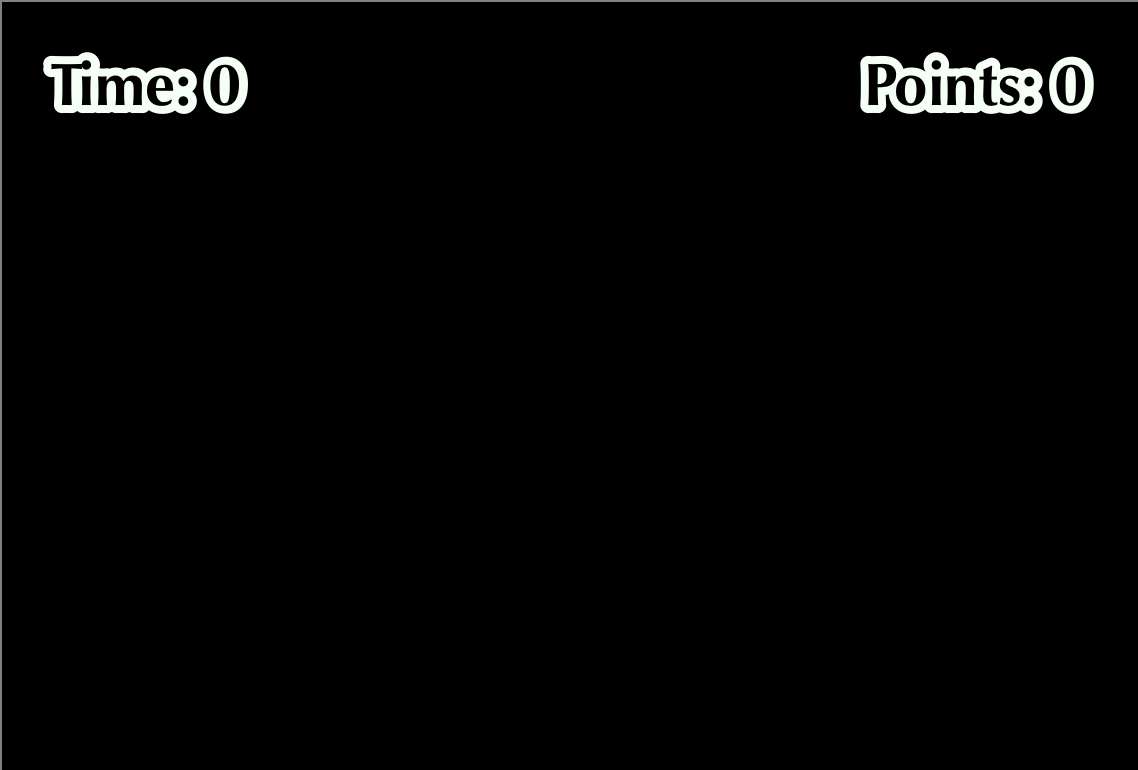
\includegraphics[width=0.5\linewidth]{images/Chapter7/timed_mode_ui.png}
\end{figure}

\subsubsection{UI for the endless game mode}
Now lets create the second UI. We'll start of by creating a new \ccbfile{}.
\begin{leftbar}
Create a new \ccbfile{} of type \textit{Layer} and name it
\textit{EndlessModeUI}. Select the root node of the new \ccbfile{} and change
the size type to be \textit{percentage of parent container} for both, width and height. Set the
values for width and height to \textit{100\%}.
\end{leftbar}
Next, let's add a label that displays the amount of seconds a player has
survived. Once again we can copy the existing label from the
\filemention{TimeModeUI.ccb} file since we want both labels to look identical.
\begin{leftbar}
Open \filemention{TimeModeUI.ccb} and copy the label in the \textbf{top left
corner}. Then open \filemention{EndlessModeUI.ccb} and paste the label. Select
the pasted label and modify it as following:
\begin{enumerate}
  \item Change the label text to \textit{Survived: 0}
  \item Set up a code connection to the \textbf{Owner var} and name it \textit{survivedLabel}
\end{enumerate}
\end{leftbar}

Besides this label we will also need to display a health bar in the endless game
mode. The easiest way to implement a health bar in \cocos{} is taking a plain
\inlinecode{CCColorNode} and scaling it depending on the current health level
of the player.

\begin{leftbar}
Drag a \textit{Color Node} from the node library to the stage. Set it up as
following:
\begin{enumerate}
  \item Select the \textit{Position Reference Corner} to be the top right corner
  \item Change the position to \textit{(20,20)}
  \item Change the anchor point to \textit{(1.0, 1.0)}
  \item Change the node color to \textit{green} (pick any color you enjoy)
  \item Change the font size to \textit{30}
  \item Set up a code connection to the \textbf{Owner var} (not the \textit{Doc
  root var}, this is very important!) and name it \textit{healthBar}
\end{enumerate}
\end{leftbar}

Now the UI for the endless mode should look like this:

\begin{figure}[H]
    \centering
    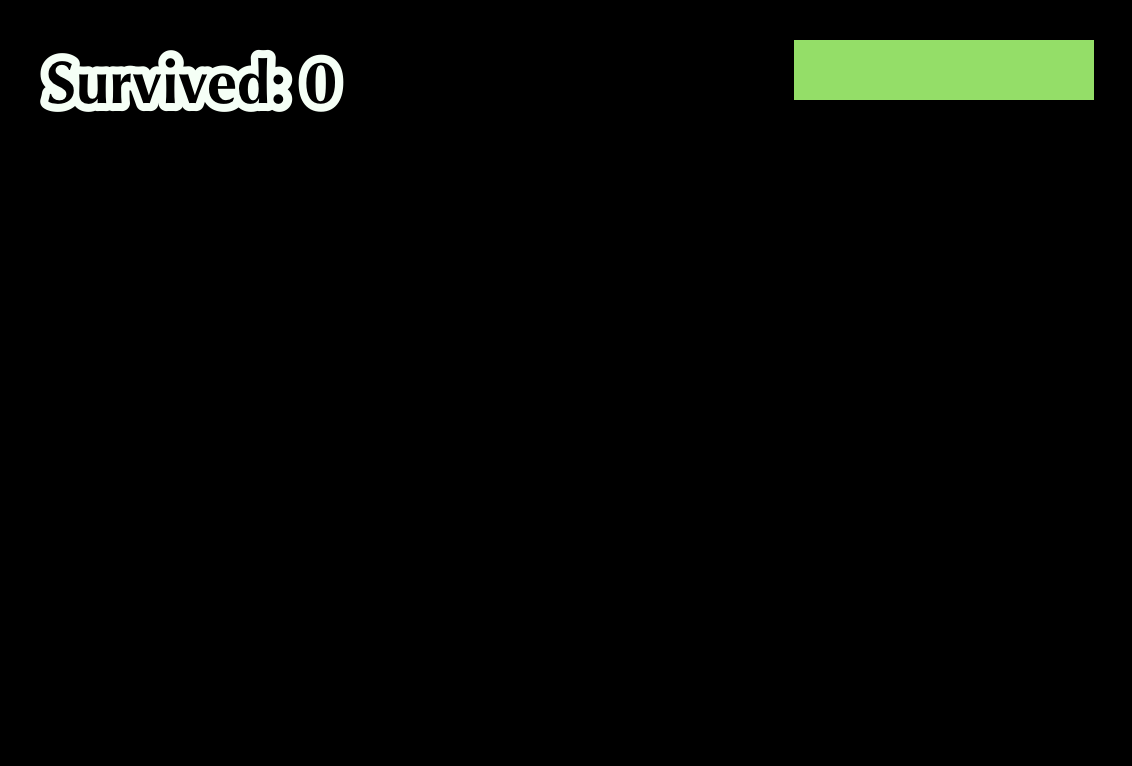
\includegraphics[width=0.5\linewidth]{images/Chapter7/endless_mode_ui.png}
\end{figure}

We're done with the UI setup. To make these score displays actually show up as
part of the game, we'll now move to implementing the two game modes in code.

\subsection{Implement game logic for different modes}
We need to change multiple parts of our game to support two different game
modes.Depending on which game mode a player selects, we want to display a different
score board and also implement a different set of rules.

Before we dive into coding, let's try to figure out what we'll need to
implement:
\begin{itemize}
  \item When we start a game, the \inlinecode{MainScene} class needs to know
  which game mode a user has selected
  \item \inlinecode{MainScene} shouldn't know
  anything about the rules of the selected game mode. That way we could add game
  modes in the future without increasing the complexity of
  \inlinecode{MainScene}
  \item Every game mode should know about its rules (when does a player earn /
  loose points, when does a game end)
  \item Every game mode should know which score board entries it has and it
  should be responsible for updating them based on the current state of the game
\end{itemize}

We should try to come up with a solution that lets us add more game modes as
easily as possible. One modular way of implementing this is setting up different
game modes as individual classes. These classes can be referenced by the
\inlinecode{MainScene} class. In this scenario, the \inlinecode{MainScene} class
remains responsible for the core of the game, it spawns falling objects (though,
even this could be moved into the gameplay classes eventually) and lets them
fall to the ground. It handles collision detection and determines if an object
was caught or dropped.

The consequences of catching or dropping objects however, are not implemented in
the \inlinecode{Gameplay} class itself. Instead, they are implemented by the
game modes. This means that the \inlinecode{Gameplay} class needs to inform the
game mode when a significant event occurs. The game mode itself can then decide
how this event impacts the gameplay.

Here's a diagram that illustrates our solution:

\begin{figure}[H]
    \centering
    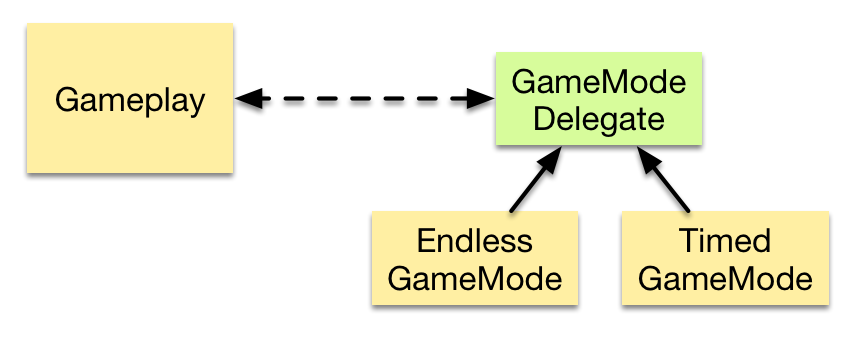
\includegraphics[width=0.5\linewidth]{images/Chapter7/gameplay_design.png}
\end{figure}

\subsubsection{Defining a protocol for game modes}
Let's start implementing this design. The first step is defining a protocol
that can be implemented by all game modes. In the diagram above I've highlighted
the protocol in green.
\begin{leftbar}
Create a new Swift file in \xcode{} and call it
\filemention{GameModeDelegate.swift}.
Then add the following protocol definition to it:
\begin{lstlisting}
typealias GameOver = Bool

protocol GameModeDelegate: class {
  var userInterface: CCNode! { get }

  func gameplay(mainScene:MainScene, droppedFallingObject:FallingObject)
  func gameplay(mainScene:MainScene, caughtFallingObject:FallingObject)
  func gameplayStep(mainScene:MainScene, delta: CCTime) -> GameOver
}
\end{lstlisting}
\end{leftbar}
Note that I have omitted the source code documentation of this protocol for the
sake of brevity. The protocol we've just defined will be implemented by
multiple classes, it's important to document its methods and properties for developers that want
to add game modes in future. You can take a look at the source code for
this chapter on GitHub() to read the documentation. %TODO: add link to source
% code

\begin{details}[frametitle={Source code
documentation in Swift}] Many details about source code documentation in Swift are still up in the air.
NSHipster provides a great article that describes the currently supported
documentation style: \url{http://nshipster.com/swift-documentation/}.
\end{details}

Let's discuss this protocol in detail. The first interesting aspect is a
\inlinecode{typealias} statement before the protocol declaration. Using
typealiases is simple in Swift, and it's a nice way of better capturing the
semantics of a type. Returning a type of \inlinecode{GameOver} is easier to
understand the returning a \inlinecode{Bool}.

The second thing to note is that we
have defined the protocol as a \textit{class-only} protocol. We can do that by
adding the \inlinecode{class} keyword to the protocol's inheritance list. Later
you'll see that any type that implements \inlinecode{GameModeDelegate} is
required to be a reference type, because we need to pass references to it to
\cocos{}.

We start our protocol by requiring a property: \inlinecode{userInterface}. This
property shall provide access to the game mode's user interface. The
\inlinecode{MainScene} class can use this property to access the UI for the
currently active game mode.
We only expose as a getter as part of the protocol, the UI cannot be changed
from outside of the game mode class. Each game mode knows the \ccbfile{} of its
UI and loads it as soon as the game mode is created.

Next, we define two methods that get called when objects get dropped or caught.
Both methods receive a reference to the \inlinecode{MainScene}. This is pretty
common when using the delegate pattern. Theoretically a game mode instance
could be the delegate of multiple \inlinecode{MainScene} instances. By passing
the the \inlinecode{MainScene} in which the event occurred to the delegate the
delegate can perform different actions based on which \inlinecode{MainScene}
called the method. The second parameter sent to both methods is the object which
has been caught or dropped. The class implementing
the \inlinecode{GameModeDelegate} can use this information to determine whether
points should be added or subtracted.

The last method(\inlinecode{gameplayStep:}) fulfills two purposes. Firstly, it
allows game modes to hook into the update method of \inlinecode{MainScene}. That
is necessary for any time based actions, e.g. capturing the total time that
has passed since the beginning of the game. The second purpose is fulfilled by
the \inlinecode{GameOver} return value. The return value allows the game mode to
tell the \inlinecode{MainScene} that the game is over. All game modes will use
this method to implement the game over condition.

Now that our protocol is defined we can implement the two game modes. 

\subsubsection{Implementing the timed game mode}
Let's start by implementing the timed game mode. Since we thought about the
software design upfront and even defined a protocol for game modes, the
implementation itself is not too complicated.

\begin{leftbar}
Create a new Swift file and name it \filemention{TimedGameMode}. Add the
following class definition to the new file:
\begin{lstlisting}
@objc(TimedGameMode)
class TimedGameMode: GameModeDelegate {
  var timeLabel: CCLabelTTF!
  var pointsLabel: CCLabelTTF!
}
\end{lstlisting}
\end{leftbar}
There's a lot going on in these few lines. Firstly, we need the
\inlinecode{@objc} annotation to make this class visible to \cocos{}. \cocos{}
is written in Objective-C and can only see classes that are subclasses of
\inlinecode{NSObject} or that have the \inlinecode{@objc} annotation. So far all
of our classes have been subclasses of \cocos{} classes, and all of them in turn
are derived from \inlinecode{NSObject}, therefore this annotation wasn't
necessary. The \inlinecode{TimedGameMode} class is our first class that is not a
subclass of an Objective-C class.

In the second line we declare that our class conforms to the
\inlinecode{GameModeDelegate} protocol. We also declare to instance variables
for the code connections that we set up in the \ccbfile{} for the timed game
mode. We have access to two different labels, one displays the player's the
other one displays the time that's left.

We'll need a whole set of additional variables. We need a
\inlinecode{userInterface} variable to conform to the
\inlinecode{GameModeDelegate}, we also need variables to store the amount of
points the player has scored and the time that is left in the current game.

\begin{leftbar}
Add the following properties and property observers to the
\inlinecode{TimedGameMode} class:
\begin{lstlisting}
let minPoints = 0
let minTime = 0.0

private(set) var userInterface: CCNode!

private var time: CCTime = 10 {
  didSet {
    updateTimeDisplay(time)
  }
}

private var points: Int = 0 {
  didSet {
    updatePointsDisplay(points)
  }
}
\end{lstlisting}
\end{leftbar}
The first two constants are used to define the bottom line for time and points
in this game mode. In almost all cases using constants should be preferred over
using numbers directly in code. By defining constants our intentions are obvious
to other developers.

Further, we add the \inlinecode{userInterface} variable. This variable will
store the loaded \ccbfile{} that belongs to the timed game mode. It is also
required to conform with the \inlinecode{GameModeDelegate} protocol.

Next, we declare and define the \inlinecode{time} property that stores the time
that is left during the current game. For testing purposes our games only last 10 seconds. We
also add a property observer. When the time value changes we call the (yet to
be implemented) \inlinecode{updateTimeDisplay:} method, that method updates the
label that displays the leftover time.

We essentially do the same for the \inlinecode{points} property.

Next, let's implement the two helper methods that update the time and point
labels.
\begin{leftbar}
Add the following two methods to \inlinecode{TimedGameMode}:
\begin{lstlisting}
func updatePointsDisplay(points: Int) {
  pointsLabel.string = "Points: \(points)"
}

func updateTimeDisplay(time: CCTime) {
  timeLabel.string = "Time: \(Int(time))"
}
\end{lstlisting}
\end{leftbar}
These methods are very simple. We only put this code into separate methods
because we need the functionality in multiple places, as you'll see shortly.

Next, before we implement the methods defined in our protocol, let's tackle the
initializer of this class. The main task the the initializer needs to perform is
loading its UI from a \ccbfile{}.
\begin{leftbar}
Add the following initializer:
\begin{lstlisting}
init() {
  userInterface = CCBReader.load("TimedModeUI", owner:self)
  updatePointsDisplay(points)
  updateTimeDisplay(time)
}
\end{lstlisting}
\end{leftbar}
In the first line we load the \filemention{TimedModeUI} \ccbfile{}. We store the
loaded node hierarchy in the \inlinecode{userInterface} property, that way it
can be accessed by \inlinecode{MainScene}.
We also call our to label helper methods, so that the labels display the correct
initial values for time and points.

Now we can move on to the core of this class. The methods that are required by
the \inlinecode{GameModeDelegate} protocol.

Let's start with the \inlinecode{gameplay(mainScene:,
droppedFallingObject:)} method. Now it's time to make some decisions on the
rules of the timed game mode. I suggest that we subtract 1 point when the player
drops an object that should be caught. Because we don't want to be too mean we
set the lowest possible score to 0.

\begin{leftbar}
Add the following method to \inlinecode{TimedGameMode}:
\begin{lstlisting}
func gameplay(mainScene:MainScene, droppedFallingObject:FallingObject) {
  if (droppedFallingObject.type == .Good) {
    points = max(points - 1, minPoints)
  }
}
\end{lstlisting}
\end{leftbar}
If the object that has been dropped is a \inlinecode{.Good} object, we subtract
one point. Using Swift's \inlinecode{max} function we make sure that the total
score never drops below \inlinecode{minPoints}, which we have defined as 0.

Next, we'll implement the method that gets called when objects are caught.
Once again time to decide on some rules. I propose to add a point when a good
object is caught and subtract a point when a bad object is caught. You can
obviously feel free to use different values!

\begin{leftbar}
Add the method for caught objects to \inlinecode{TimedGameMode}:
\begin{lstlisting}
func gameplay(mainScene:MainScene, caughtFallingObject:FallingObject) {
  switch (caughtFallingObject.type) {
  case .Bad:
    points = max(points - 1, minPoints)
  case .Good:
    points += 1
  }
}
\end{lstlisting}
\end{leftbar}
Since we are checking for multiple possible values of an enum using a switch
statement results in nicely readable code. Besides the switch statement the
implementation is pretty straightforward.

Now there's only one last method to implement:
\inlinecode{gameplayStep(mainScene:, delta:)} We need to do two things in the
implementation of this method:
\begin{enumerate}
  \item Subtract passed time from time that is left over
  \item Check if time reached minimum time (0.0) and return \inlinecode{true} if
  that's the case
\end{enumerate}
\begin{leftbar}
Add the following implementation of the step method to
\inlinecode{TimedGameMode}:
\begin{lstlisting}
func gameplayStep(mainScene: MainScene, delta: CCTime) -> GameOver {
  time -= delta
  return !(time > minTime)
}
\end{lstlisting}
\end{leftbar}
First, we subtract \inlinecode{delta} from the remaining game time. Next, we
check if the total time is over or not and return a \inlinecode{GameOver} value
based on that.

Congratulations! We have fully implemented our first game mode.

\subsection{Adding a game end popup}

 